% ******************************* PhD Thesis Template **************************
% Please have a look at the README.md file for info on how to use the template

\documentclass[a4paper,12pt,times,authoryear,oneside,print,index,custommargin]{Classes/PhDThesisPSnPDF}

% ******************************************************************************
% ******************************* Class Options ********************************
% *********************** See README for more details **************************
% ******************************************************************************

% `a4paper'(The University of Cambridge PhD thesis guidelines recommends a page
% size a4 - default option) or `a5paper': A5 Paper size is also allowed as per
% the Cambridge University Engineering Deparment guidelines for PhD thesis
%
% `11pt' or `12pt'(default): Font Size 10pt is NOT recommended by the University
% guidelines
%
% `oneside' or `twoside'(default): Printing double side (twoside) or single
% side.
%
% `print': Use `print' for print version with appropriate margins and page
% layout. Leaving the options field blank will activate Online version.
%
% `index': For index at the end of the thesis
%
% `draftclassic': For draft mode without loading any images (same as draft in book)
%
% `draft': Special draft mode with line numbers, images, and water mark with
% timestamp and custom text. Position of the text can also be modified.
%
% `abstract': To generate only the title page and abstract page with
% dissertation title and name, to submit to the Student Registry
%
% `chapter`: This option enables only the specified chapter and it's references
%  Useful for review and corrections.
%
% ************************* Custom Page Margins ********************************
%
% `custommargin`: Use `custommargin' in options to activate custom page margins,
% which can be defined in the preamble.tex. Custom margin will override
% print/online margin setup.
%
% *********************** Choosing the Fonts in Class Options ******************
%
% `times' : Times font with math support. (The Cambridge University guidelines
% recommend using times)
%
% `fourier': Utopia Font with Fourier Math font (Font has to be installed)
%            It's a free font.
%
% `customfont': Use `customfont' option in the document class and load the
% package in the preamble.tex
%
% default or leave empty: `Latin Modern' font will be loaded.
%
% ********************** Choosing the Bibliography style ***********************
%
% `authoryear': For author-year citation eg., Krishna (2013)
%
% `numbered': (Default Option) For numbered and sorted citation e.g., [1,5,2]
%
% `custombib': Define your own bibliography style in the `preamble.tex' file.
%              `\RequirePackage[square, sort, numbers, authoryear]{natbib}'.
%              This can be also used to load biblatex instead of natbib
%              (See Preamble)
%
% **************************** Choosing the Page Style *************************
%
% `default (leave empty)': For Page Numbers in Header (Left Even, Right Odd) and
% Chapter Name in Header (Right Even) and Section Name (Left Odd). Blank Footer.
%
% `PageStyleI': Chapter Name next & Page Number on Even Side (Left Even).
% Section Name & Page Number in Header on Odd Side (Right Odd). Footer is empty.
%
% `PageStyleII': Chapter Name on Even Side (Left Even) in Header. Section Number
% and Section Name in Header on Odd Side (Right Odd). Page numbering in footer

% Uncomment to change page style
%\pagestyle{PageStyleII}

% ********************************** Preamble **********************************
% Preamble: Contains packages and user-defined commands and settings
\ifsetCustomMargin
  \RequirePackage[marginparwidth=25mm, % TODO: Remove this before submitting
  left=31mm,right=31mm,top=31mm,bottom=31mm]{geometry}
  \setFancyHdr % To apply fancy header after geometry package is loaded
\fi


\raggedbottom

\usepackage[edges]{forest}


\usepackage{comment}

\usepackage[ruled,vlined]{algorithm2e}
\RequirePackage[labelsep=space,tableposition=top]{caption}
\renewcommand{\figurename}{Fig.} 
\usepackage{subcaption}
\usepackage{booktabs}
\usepackage{multirow}
\usepackage{siunitx} 
\ifuseCustomBib
   \RequirePackage[square, sort, numbers, authoryear]{natbib}
\fi

\renewcommand{\bibname}{References}
\DeclareMathOperator{\sign}{sign}
\DeclareMathOperator{\turns}{turns}
\DeclareMathOperator{\avg}{Avg}
\setcounter{secnumdepth}{2}
\setcounter{tocdepth}{2}

% ************************ Thesis Information & Meta-data **********************
% Thesis title and author information, refernce file for biblatex
\title{Reinforcement Learning Meets Balls into Bins}




\subtitle{Part II, Computer Science Tripos}
\author{Andor Vári-Kakas}
\dept{Department of Computer Science and Technology}
\university{University of Cambridge}
\renewcommand{\crest}{}
%\crest{
\includegraphics[width=0.2\textwidth]{University_Crest}}
\renewcommand{\submissiontext}{}
\college{Churchill College}



% ***************************** Abstract Separate ******************************
% To printout only the titlepage and the abstract with the PhD title and the
% author name for submission to the Student Registry, use the `abstract' option in
% the document class.

\ifdefineAbstract
 \pagestyle{empty}
 \includeonly{Declaration/declaration, Abstract/abstract}
\fi

% ***************************** Chapter Mode ***********************************
% The chapter mode allows user to only print particular chapters with references
% Title, Contents, Frontmatter are disabled by default
% Useful option to review a particular chapter or to send it to supervisior.
% To use choose `chapter' option in the document class

\ifdefineChapter
 \includeonly{Chapter3/chapter3}
\fi

% ******************************** Front Matter ********************************
\begin{document}
\frontmatter

\maketitle

%%% ******************************* Thesis Dedidcation ********************************

\begin{dedication} 

I would like to dedicate this thesis to my loving parents \dots

\end{dedication}
% ******************************* Thesis Declaration ***************************

\begin{declaration}
I, Andor Vari-Kakas of University of Cambridge, Churchill College, being a candidate for Part II of the Computer Science Tripos, hereby declare that this dissertation and the work described in it are my own work, unaided except as may be specified below, and that the dissertation does not contain material that has already been used to any substantial extent for a comparable purpose. I am content for my dissertation to be made available to the students and staff of the University.
% Author and date will be inserted automatically from thesis.tex \author \degreedate
\end{declaration}
%%\begin{acknowledgements}      


I would like to thank my supervisors, Dr Thomas Sauerwald and Dimitris Los, for their enthusiasm and the long hours of discussions. I would also like to thank Viktória Csizmadia, Dr John Fawcett, Gábor Pituk, Zoltán Molnár-Sáska and Radzim Sendyka for their valuable feedback. And finally, I am thankful to my family for their never-ending support.


\end{acknowledgements}


% ************************** Thesis Acknowledgements **************************

\begin{proforma}      


\begin{table}[h]
\begin{tabular}{ll}
Candidate Number:  & 2433E \\
College: & Churchill College \\
Project Title:    &  Reinforcement Learning meets Balls-into-Bins  \\
Examination:  & Computer Science Tripos - Part II, May 2022   \\
Word Count:  & 0  \\
Lines of Code: & 0 \\
Project Originator: & Dr Thomas Sauerwald, Dimitris Los \\
Supervisors: & Dr Thomas Sauerwald, Dimitris Los 
\end{tabular}
\end{table}
\NOTE{A}{Replace 0 with actual numbers.}

\section*{Original Aims of the Project}

The original aim of the project was to explore the applicability of Reinforcement Learning methods to optimising load balancing protocols. In particular, to find suitable decision strategies for parametric balls-into-bins protocols, which are abstractions of randomised load balancing.

\section*{Work Completed}

I have completed the success criteria, by investigating Reinforcement Learning approaches to different balls-into-bins protocols, contrasting them with dynamic programming and heuristic algorithms, and analysing them all in a modular, easy-to-use environment. As extensions, the behaviour of the strategies have been analysed, and several lemmas and conjectures have been formulated.

\section*{Special Difficulties}

None.

\end{proforma}

%%% ************************** Thesis Abstract *****************************
% Use `abstract' as an option in the document class to print only the titlepage and the abstract.
\begin{abstract}
This is where you write your abstract ...
\end{abstract}


% *********************** Adding TOC and List of Figures ***********************

\tableofcontents

\listoffigures
\listoftables

% \printnomenclature[space] space can be set as 2em between symbol and description
%\printnomenclature[3em]

\printnomenclature

% ******************************** Main Matter *********************************
\mainmatter

\chapter{Introduction}\label{introduction}

\ifpdf
    \graphicspath{{Chapter1/Figs/Raster/}{Chapter1/Figs/PDF/}{Chapter1/Figs/}}
\else
    \graphicspath{{Chapter1/Figs/Vector/}{Chapter1/Figs/}}
\fi


\section{Motivation}

Load balancing has been an important topic for many years, and it has gained even more attention recently e.g.\ cloud computing ~\cite{mishra2020cloud}. In the usual setup, there are some servers, and whenever a job arrives, the goal is to allocate it to one of the servers such that no server is overloaded (which at high burden often requires also that no server is underloaded). At first glance, it might seem an easy problem to solve: always allocate the job greedily to the currently least loaded server. Or even simpler, in the case of homogeneous jobs: apply round-robin scheduling to the servers, using each of them in a cyclic way. 

The problem with these approaches is that they require a centralised load balancer. That central load balancer would be a single point of failure, reducing the robustness of the whole system, and decreasing performance due to its sequential nature\NOTE{D}{This is a very important point. For some applications, e.g., searching at Google, you cannot have all requests going through a single machine.}. An alternative is to use randomised load balancing. The idea is to allocate the jobs according to a random protocol -- the simplest being choosing a server uniformly at random -- that can be run independently on each client (requesting the job), without a central load balancer. The obvious question is how to shape this random protocol such that a good balance is achieved. A groundbreaking result in this topic was presented in ~\cite{azar1999twochoice}. They showed that the \TwoChoice protocol, which always randomly queries the load of two independent servers, and allocates the job into the lesser loaded of the two, achieves a maximum load of $\frac{\ln(\ln(n))}{\ln(2)} + O(1)$ after $n$ jobs, with high probability (meaning that as $n$ goes to infinity, the probability converges to $1$). This result led to extensive further study of the topic (see e.g.\ ~\cite{richa2001surveytwochoice}), and even large companies, such as Twitter started using this idea (often called ``The power of Two-Choices'') ~\cite{anderson2019twitter}.


There are various versions of the load balancing problem (e.g.\ homogeneity of the jobs, random protocol used), and so for consistency reasons, the research community adapted the following standard abstraction: the servers are bins, and the jobs are balls. This is what I will use in the later chapters as well. This has the further advantage, that random protocols such as \TwoChoice have proved to be useful outside the field of load balancing too, e.g.\ hashing ~\cite{azar1999twochoice}. See ~\cite{udi2017ballsintobinslandscape} for a comprehensive survey. I will provide a more rigorous definition of the balls-into-bins abstraction in Chapter ~\ref{preparation}.


There are other random protocols suggested, that are more realistic, or more efficient than \TwoChoice in some circumstances.\NOTE{D}{Maybe start with stating which assumptions are unrealistic for load balancing using two-choice.} For example, we can see that if both of the bins queried by \TwoChoice have very low load, then, it was unnecessary to query both (e.g.\ communication overhead, slows down servers), and only one of them would be enough. \OneChoice, however, which simply allocates the ball uniformly at random (``takes 1 sample and accepts that'') has been shown to have exponentially worse maximum load (see e.g.\ the Randomised Algorithms course), so it is not sufficient. Something in the middle is \TwoThinning ~\cite{feldheim2021thinning}, which samples one bin (``primary bin''), and either accepts that, or concludes that is has too high load, in which case the ball is allocated uniformly at random into one of the bins.\NOTE{D}{See email for the two interpretations of thinning.} This, on average, requires less than $2$ queries per ball, but it requires a decision strategy (or just ``strategy'') for whether to accept or reject a bin. This dissertation is about optimising such strategies in protocols like \TwoThinning, which I will call ``parametric protocols'' as they all require some extra input, usually a decision strategy. The goal is to optimise some objective function measuring how ``balanced'' the load distribution is, such as the maximum load of the bins after some number of balls have been allocated.



\section{My approach}

For finding good strategies, I will compare Reinforcement Learning (RL) methods with more classical approaches (e.g.\ dynamic programming) and other heuristics (e.g.\ mean thinning). RL is a natural choice, since we have to make optimal decisions (``choose ideal threshold for accept/reject'') in a dynamic, stochastic process. RL is based on collecting rewards, and a first idea could be getting a reward only after all the balls have been allocated (end of an execution), based on the final load distribution. There is more refinement needed, however, to make it work properly, which I will discuss in later chapters. RL has already been applied to load balancing in the literature, mostly related to networking ~\cite{attiah2020RLcellular}, ~\cite{yeo2021controller}, but they use an abstraction slightly different from the balls-into-bins mode. The parametric balls-into-bins protocols I will study received much attention in the academic community only recently, though there have been earlier, mostly empirical studies as well (see. e.g.\ ~\cite{derek1986twothinningfirstattempt}). At the moment, there are strategies (e.g.\ for \TwoThinning) that are proven to achieve optimal results up to a constant factor ~\cite{feldheim2021thinning}, but only for very large values of balls and bins (the results are almost exclusively ``asymptotic''). Therefore, these results are of less help directly in real-world scenarios, where there are much less number of jobs and servers. There are $3$ reasons why most of these theoretical results are not applicable for small values: 1) the inequalities in the proofs don't work for small values ~\cite{feldheim2021longtermthinning} so the theoretical guarantees might not hold, 2) the constant factor overhead in the result is significant and 3) suggested \textit{positive} integer parameter values used by the strategy would equal to $0$, e.g.\ $\floor{\ln(\ln(\ln(nunber\: of \: servers)))}$ which is usually $0$ even for large datacenters ~\cite{uzaman2019datacentersize}.

\NOTE{D}{What about the two-thinning paper by Feldheim? or Mean-Thinning?}


Looking at the practical application of the \TwoThinning protocol, it is often much more natural and effective if the queried server itself decides whether to take the job, rather than sending back its current load value back to the client which makes the decision whether to accept of reject that server.  Overall, the process is 1) the client chooses a server uniformly at random, 2) the server either completes the job or passes it on to a server chosen uniformly at random.

The important question left is what information can the server use in deciding whether to accept a job or not. It needs some ``reference'' to assess its load relative to others, which requires some centralised information. There are several options, for example the servers could maintain the overall load of the system, or they could synchronise their individual loads from time-to-time (see e.g.\ ~\cite{zhang2018datacenterloadbalancing} for efficient communication in data centers). I will focus on the latter, which crucially allows a server to make its decision based on the (possibly slightly outdated) loads of all the other servers. When a server decides to pass on the job to another one, the motivation for choosing the other server at random is that due to parallelism and the possibly outdated information, the seemingly least loaded server could quickly become the most overloaded if all the other servers pass the jobs to that one.


Having introduced the practical details, I will take a more theoretical approach in this project. Realising the lack of exact, non-asymptotical results even for simple settings, and to simplify the analysis, I will try to solve a simpler problem than the practical one presented above: the strategy is given the \textbf{exact load distribution} at the moment, and it is offered a specific (``primary'') bin, which it can either accept and place the ball there, or reject, in which case the ball is allocated to a ``secondary'' bin chosen uniformly at random. Another big simplification is that all the balls are allocated by a single instance of the strategy sequentially, i.e.\ the load distribution depends only on its own allocations. We will see that finding a good strategy even for this greatly simplified version proves to be very challenging for RL and other algorithms. When describing the candidate strategies I will highlight those that are more directly applicable in more realistic scenarios. \NOTE{A}{This is the single most important paragraph in the dissertation! Check if it is 100\% clear to the reader, both the motivation and the simplified problem.}


Overall, the intention of this dissertation is more to survey the applicability of RL and other approaches in different settings, than to provide directly practical protocols. Another aim of the project is to gain a deeper insight to how an optimal strategy looks like.
\NOTE{D}{I don't think you have put serious effort in highlighting the merits and results of your work in the above paragraph. Andor: This comment always makes me smile for some reason when I read it, so I don't delete it :) .}

\NOTE{D}{As discussed in the last meeting, even the non-RL setting you give it a load distribution and the NN needs to pick a threshold that will be used for the next $K$ steps is interesting, because it could work in a batched setting. Andor: what should I do with it?}


\section{Outline}

The outline of the dissertation is as follows.


In Chapter ~\ref{preparation}, I define the terms of the balls-into-bins terminology more precisely, and also make the underlying assumptions explicit. Then, I describe the balls-into-bins protocols that I will analyse in later chapters -- I do not discuss all of them at such length as I did in this chapter for \TwoThinning, but similar practical considerations apply\NOTE{A}{Is this sentence needed?}. Finally, I explain the basics of RL, with particular focus on Deep Q-Learning, which is the main algorithm that I used.


In Chapter ~\ref{implementation}, I explain the implementation details of RL and ``classical'' algorithms such as dynamic programming, for learning strategies for various parametric protocols. I also list several extensions of the simple RL algorithms that I implemented for better results, e.g.\ reward shaping. Finally, I explain the code structure with the extensible object-oriented style in focus.


In Chapter ~\ref{evaluation}, I compare the implemented approaches from different aspects, including how well they can balance the load, and their training complexity (if any). I also provide a thorough hyperparameter analysis for RL. As an extension, I analyse the behaviour of the different strategies. \NOTE{A}{Is it an extension?...}


In Chapter ~\ref{conclusion} I conclude with some future work ideas for improving the RL approaches, gaining better insights to optimal strategies, and extending the study to different settings.
\chapter{Preparation}\label{chapter2}

\ifpdf
    \graphicspath{{Chapter2/Figs/Raster/}{Chapter2/Figs/PDF/}{Chapter2/Figs/}}
\else
    \graphicspath{{Chapter2/Figs/Vector/}{Chapter2/Figs/}}
\fi


%!TEX root = ../thesis.tex
\chapter{Implementation}\label{implementation}

\ifpdf
    \graphicspath{{Chapter3/Figs/Raster/}{Chapter3/Figs/PDF/}{Chapter3/Figs/}}
\else
    \graphicspath{{Chapter3/Figs/Vector/}{Chapter3/Figs/}}
\fi


\section{Two-Thinning}


\subsection{Deep Q-Learning Implementation}


Unlike for many supervised learning problems, there is no library for RL that provides one-liner solutions to my settings. While there are some libraries for RL (e.g. Stable Baselines, Pyqlearning), they are usually very hard to customize, and for example the format of the state space is very unique RL problems. Also, implementing the basic RL logic is not too long, so I made the decision to implement the RL logic myself, and use Pytorch for the NNs.


\NOTE{A}{At this point I expect the reader to understand Deep Q-Learning in enough detail, so that I just have to note some implementation details.}


\subsubsection{Deep Q-Network (DQN)} \label{DQN}


The NN used in Deep Q-Learning is often referred to as Deep Q-Network (DQN). 


There are two ways to formulate the \textsc{Two-Thinning} setting as a MDP. One is to treat (load vector, primary bin) pairs as states, and accept/reject as actions. The other is to treat load vectors as states, and thresholds for accepting/rejecting as actions. The latter implicitly makes use of a very important (also intuitive) property of an optimal policy:


\begin{lemma} \label{lemma: thresholdproperty}
At a load vector $v$, the optimal policy doesn't reject a primary bin with load $x$, if it would accept a primary bin with load $y>x$. That is, the optimal strategy is always a threshold strategy, that rejects above a load value $z$ and accepts otherwise.
\end{lemma}


\NOTE{A}{Add proof, or say something about it.}

Since this lemma holds, I chose the second formulation, which using this lemma, restricts the space in which the algorithm has to search for the optimal policy. We will see later that this lemma is useful in optimising the dynamic programming approach as well.


Therefore the input to the DQN is a load vector $v$, and the output is an estimate of $Q(v, a)$ for each possible thresholds. There is no point in using non-integer thresholds, since the load of the primary bin is always a non-negative integer. Also, there is no benefit in using a threshold larger than the current maximum load, as setting the threshold to that instead achieves the same (accepting everything). Similarly, as a consequence of Lemma \ref{lemma: thresholdproperty} \NOTE{A}{Is it a corollary strictly speaking?}, the best possible load primary bin load is $0$, therefore it never makes sense to reject it (or in general reject a bin with minimum load). So theoretically, the possible thresholds should be from $0$ to $m$, that is, the output of the DQN should have size $m+1$. Even though it is possible that a load of $m$ is reached during execution, it has a very small probability (more details in Chapter \ref{evaluation}), so I decided to restrict the maximum threshold available for the algorithm. The optimal maximum threshold should depend on $n$ and $m$, and together with other hyperparameters, I provide their final values and their importance in later sections. 


Now that the output of the DQN is fixed, the other question is how to represent the input to the DQN, which is a load vector $v$. First of all, I always sort the load vector before feeding it into the network. This is possible because the order of the bins doesn't matter in \textsc{Two-Thinning}, unlike in \textsc{Graphical Two-Choice}. This sorting makes the function that the network has to learn easier (it doesn't have to learn permutation invariance), and it will be important when using RNN as the architecture. Then, I one-hot encode each load value independently. The motivation for this is that NNs often can't learn well with ordinal data - they would think that the load values are on a continuous scale, but in fact, the real difference between e.g. load $0$ and $1$ is much smaller than the real difference between load e.g. $m-1$ and $m$. \NOTE{A}{https://stats.stackexchange.com/questions/423820/do-ordinal-variables-require-one-hot-encoding}. The natural range of one-hot encoding for the load values is from $0$ to $m$, but to condense the input to the network (and hence reduces the number of weights to train) I tried collapsing the very high load values with very small probability, into one ``outlier'' class. This didn't provide better results, so I do not discuss it any further.


Now that the input and output format is laid down, I turn to the discussion of the architecture of the DQN. From the load values in a load vector, the highest ones are much more important, since we care about minimising the maximum load. On the extreme, if the bin with the maximum load had one more ball in it, that would be more significant than if an average bin had one more ball in it. Hence, my idea was to process the load vector in increasing order of the loads, that is, in increasing order of importance. For this, using an RNN is a perfect choice. It is used for processing sequential input, and what is more, by the end it forgets the earlier inputs to some extent, and therefore focuses more on the final (in our case most important) inputs, as desired. As mentioned in Chapter \ref{preparation}, there are more complex versions of RNNs, whose main advantage is that they forget less. However, as this forgetting property is desirable in our case, this advantage is not really an advantage. On the other hand, they are less susceptible to the vanishing/exploding gradient problems \cite{noh2021rnnvanishinggradient}, so they are sometimes easier to train, therefore I tried GRU and LSTM as well, but they didn't provide additional benefits, so I will stick to the vanilla RNN. After the last input, we can extract the hidden state of the RNN, whose exact size I will discuss in the hyperparameters section. To get the output, the estimated $q(v,a)$ values for each possible threshold $a$, I apply some (as for other hyperparameters, I discuss the exact values later) fully convolutional (linear) layers on the final hidden state of the RNN. These linear layers not only bring the output to the correct shape, they also transform from the internal representation of the RNN to the space of the action-values. \NOTE{A}{Explain some more?}\NOTE{A}{Add a figure about the DQN architecture.}. As for the activation functions, I use a ReLU activation between the fully convolutional layers, and the tanh activation inside the RNN, following common practice \cite{szandala2020activationfunctions}.


\subsubsection{Stabilising Training}


In practice, Deep Q-Learning - and in general any off-policy deep reinforcement learning algorithm - can become unstable during training. There are several methods proposed to address this issue, out of which the three most popular are the following. I added these to my implementation as well.


\paragraph{Experience Replay}


Experience replay was first introduced in \cite{lin1992experiencereplay}. The problem it is trying to solve is that in vanilla Deep Q-Learning, subsequent the update steps are correlated - i.e. in our case, after we update network around a load vector with $x$ balls, we next update it around a load vector with $x+1$ balls. This correlation stems from updating in the same order as executing the actions in the game. In order to get the theoretical guarantees for these supervised learning-like updates, we need to have independent identically distributed, so certainly not correlated training samples. The idea in experience replay, is to instead of calling the update rule \ref{eq:deep-q-learning-update-with-semi-gradient} on the current $(s, a, s', r)$ tuple, we store this tuple in an experience replay buffer. Then, after every fixed number of steps, a batch of tuples are samples uniformly at random from the buffer, and the DQN is updated according to those tuples. Another benefit of the idea is that tuples can be reused multiple times, leading to a more efficient learning. Nevertheless, there is a size limit on the buffer to get rid of outdated samples, so whenever it is full, a tuple is deleted from it. I implemented it using a deque data structure. Finally, note the importance of sampling a batch of tuples when updating, and not only a single tuple - it has been shown that batching helps stabilising learning \cite{qian2020batchingsgd}.


\paragraph{Target Network}


The idea of a target network was first introduced in \cite{argueta1992targetnetwork}. The main difference between Q-Learning and Deep Q-Learning is that in the former, during one step we only update a single value in the Q-table, while in the latter, due to the nature of NNs, many neighbouring values are also updated (it is a continuous function approximation). This becomes problematic, since looking at the update rule \ref{eq:deep-q-learning-update-with-semi-gradient} for Deep Q-Learning, to update at a Q-value $Q_{\mathbf{w_t}}(s_t, a_t)$, a neighbouring Q-value $Q_{\mathbf{w_t}}(s_{t+1}, a')$ is used. This can lead to a blow-up in the Q-values, intuitively, as a chain reaction. \NOTE{A}{Honestly, I don't understand it at all... I couldn't find any good explanation of this.}. The idea with target networks, is to have two copies of the same network architecture: one whose weights are updated by the update rule, and one that provides $Q_{\mathbf{w_t}}(s_{t+1}, a')$ of the ``target'' part $r_{t+1}+ \max_{a'} Q_{\mathbf{w'_t}}(s_{t+1}, a')$ of the rule. This weights $w'$ of the target network are updated to that of the main network periodically, every fixed number of training episodes.


\paragraph{Using a better Optimiser}


Looking more closely at the update rule \ref{eq:deep-q-learning-update-with-semi-gradient}, and using the batching technique outlined for experience replay, we can see that this resembles the update rule of the Stochastic Gradient Descent (SGD) optimiser method. Therefore, instead of SGD, we could use any other optimiser method. In practice, the most widely used optimiser for Deep Q-Learning is the ADAM optimiser \cite{kingma2015adamoptimiser}. Briefly, it is a more complex version of SGD that doesn't use the raw gradients, and instead keeps track of moving averages and variances of the gradients, to adjust the step size in the size of the current gradient. An important parameter of ADAM is its learning rate, which I will optimise using hyperparameter optimisation. Also, a widely used extension in deep reinforcement learning is gradient clipping, which doesn't allow absolute gradient values to go above $1$, and has been shown to speed up training \cite{zhang2020gradientclipping}. I added gradient clipping to my implementation.\\



There are plenty of more ideas in the literature to improve the training of DQN, for example the so-called double learning \cite{hasselt2010doubleqlearning}, which argues that vanilla (deep) Q-Learning overestimates the action values, since under the hood it uses $\mathbb{E}[\max_a(Q(s,a)]$ and not $\max_a(\mathbb{E}[Q(s,a)])$. I do not consider these possibilities any further.


\subsection{Deep Sarsa-Learning Implementation}


\NOTE{A}{Maybe not needed? I don't have too many words left to use. Also, this is nothing special really.}


\subsection{Ideas Implemented for Improvement} \label{improvementideas}


In this section I outline ideas independent of DQN that I used to improve the performance of my RL algorithm. Some of these are well-known general ideas in RL, while others are specific to the \textsc{Two-Thinning} Balls into Bins setting. I will highlight why each of the ideas were worth considering for this setting.


\subsubsection{Reward Shaping} \label{rewardshaping}


As discussed in Chapter \ref{preparation}, the most direct way to formulate the \textsc{Two-Thinning} setting as a MDP is to only give reward after a final state, i.e. when all the balls have been placed. The problem with this is that rewards are very sparse - concretely, the agent only receives one reward per execution. It is problematic because until the final rewards propagate back to earlier states (that is, load vectors with few balls), the updates at earlier states are not justified - they use a zero reward and a randomly initialised next state to update the current state. Hence, the idea is to inject additional rewards into the MDP, while maintaining correctness: the optimal policy for the new modified MDP has to be optimal for the original one as well, and hence for \textsc{Two-Thinning} too. There is a very neat results proved in \cite{ng1999rewardshaping} about exactly what extra rewards can be used while maintaining the correctness property: the extra reward, when moving from state $s$ to state $s'$ using action $a$ has to be in the form $\Phi(s')-\Phi(s)$, i.e. the difference of the so-called potential functions of the two states. Intuitively, the potential function should denote an estimate of how good a state is with respect to the original (in our case final) rewards. I experimented with several candidate potential functions, and here I present the most promising ones, while I compare them numerically in the hyperparameter optimisation section \NOTE{A}{I write this sentence too many times...}.


\begin{itemize}
    \item
    $\Phi(v)=-maxload(v)$. This is a natural extension of the final reward, which is also the same expression. In practice, it turns into getting a reward $-1$ if the current ball has been allocated such that the max load has increased, and otherwise still no reward.
    \item
    $\Phi(v)=-std(v)$, where $std(v)$ is the standard deviation of the load vector. This is an extension of the previous idea, which differentiates between cases when the max load hasn't increased - it is much better if the ball is allocated in the most underloaded bin than if in the second most overloaded.
    \item
    $\Phi(v)=\sum_{x\in v} e^{\alpha * (x - avg(v))}$, where $\alpha$ is a hyperparameter. The motivation for this is similar to the previous one. This function is called the exponential potential function, and it has first been introduced as a useful tool in proving bounds for Balls into Bins settings \cite{ghosh1999exponentialpotential} \NOTE{A}{I feel that I have way too many entries in the bibliography overall, and I am not reusing them efficiently.}. As a relevant example, if the exponential potential of a load vector $v$ is $O(len(v))$, it follows that $maxload(v) < (avg(v)+log(len(v)))$.
\end{itemize}


\subsubsection{Curriculum Learning}



The idea of curriculum learning \cite{bengio2009curriculumoriginal} is to first provide easier problems to the agent, and just gradually increase the difficulty up to the original problem - just like how humans learn using a curriculum. Without curriculum learning, the agent cannot learn as much as desired from the hard problems initially \NOTE{A}{Explain some more?}. For \textsc{Two-Thinning}, I implemented curriculum learning by first starting from $m-1$ balls already being allocated, then starting from $m-2$ balls already being allocated, and so on until starting from the original empty bins. To choose the training samples on level $k$ (i.e. how to place the initial balls), I had to find which load vectors with sum $m-k$ are ``relevant'' - there are exponentially many ways to place $m-k$ balls into $n$ bins, so it is not feasible to give each of them to the agent. I decided to run the vanilla \textsc{One-Choice} protocol with $m=m-k$ balls, and it provides training samples distributed according to their occurrence when running \textsc{One-Choice}, which is a good approximation to the relevant load vectors for \textsc{Two-Thinning}. I decided to run the same amount of iterations on each level, since though there are many more different load vectors with sum $m-1$ than with sum $0$, running from the empty bins will also reach sum of loads $m-1$ but not vice versa. It is important to note that curriculum learning can serve as a pretraining phase as well. This is exactly what I did - I ran curriculum learning, and then I ran the normal training phase, which is basically just continuing with strating from the empty bins. I will analyse the effect of pretraining together with the other hyperparameters.




\subsubsection{Normalised Load}


An important difference between my work and most of the research papers, is that they use normalised load values: when they refer to a load $x$ or a threshold $a$ at a load vector $v$, the actually mean $x-avg(v)$ and $a-avg(v)$. I found it more intuitive to use real load an threshold values in my explanations, but using normalised values can make convergence during training faster, since the constant zero threshold is already a reasonable strategy (also called ``mean-thinning'') in the normalised space. On the other hand, the constant zero threshold in the original space would mean rejecting everything, which leads to \textsc{One-Choice} that has been shown to perform poorly. I will analyse the effect of training in the normalised domain together with other hyperparameters.


\NOTE{A}{Make a section about rare change, a.k.a. the batched setting?}

\subsection{Dynamic Programming}


For smaller values of $n$ and $m$ we can use dynamic programming based on the Bellman equation \ref{eq:bellmanState} to get the exact optimal policy. In general, dynamic programming approaches for RL problems are infeasible even for very small state spaces, but in this special case there are several insights that lead to a speed-up, and make it feasible for a broader set of $n$,$m$:


\begin{itemize}
    \item 
    As we did for the DQN, we can reduce the state space by around a factor of $n!$, by treating permutations of a load vector the same state, i.e. using only sorted load vectors as states.
    \item
    While a general RL problem can contains cycles in the state transition graph (that is, the agent can possibly move around a loop), in this case it is a Directed Acyclic Graph (DAG) - the next state always has exactly one more ball allocated. This is important, since we don't need to perform a fixed point iteration \cite{rhoades1991fixedpointiteration}, we can directly calculate the values based on a recurrence relation (see below).
    \item
    We can exploit Lemma \ref{lemma: thresholdproperty}: instead of using one dynamic programming state for each $Q(s,a)$ (storing a boolean value in each of them), we will have states of the form $V(s)$ (storing the optimal threshold in each of them). I also implemented a slower version of dynamic programming without using this lemma, on which interestingly I could test the validity of the lemma for specific values of $n$ and $m$.
\end{itemize}


Denoting $s[i]$ as the $i$th smallest load value in the load vector $s$, and $e_j$ as the corresponding unit vector $(0, 0, ... , 1, ..., 0, 0)$:

\begin{equation} \label{eq:twothinning-dynamicprogramming}
\begin{split}
    V_{\pi^*}(s) &= \max_a \mathbb{E} [r_{t+1} + V_{\pi^*}(s_{t+1}) \mid s_t=s, a_t=a] \\
    &= \max_{i \in [n]} \mathbb{E} [r_{t+1} + V_{\pi^*}(s_{t+1}) \mid s_t=s, a_t=s[i]] \\
    &= \max_{i \in [n]} (\sum_{0\leq j \leq i} \frac{1}{n}*V_{\pi^*}(s+e_j) + \frac{n-i-1}{n} * \sum_{j \in [n]} \frac{1}{n}*V_{\pi^*}(s+e_j))
\end{split}
\end{equation}

where we used the fact that $r_{t+1}=0$ for non-final states, and that it suffices to use only thresholds that are equal to one of the load values. Since there are many possible final states, which serve as the base cases of the dynamic programming algorithm, it was more convenient to implement is using recursion and memoisation. The base cases are those load vectors $s$ that have all $m$ balls allocated, and for those we have $V_{\pi^*}(s)=-maxload(s)$. \NOTE{A}{Exchange the last two sentences?}


We can observe that having already calculated $(\sum_{0\leq j \leq i} \frac{1}{n}*V_{\pi^*}(s+e_j) + \frac{n-i-1}{n} * \sum_{j \in [n]} \frac{1}{n}*V_{\pi^*}(s+e_j))$ for $i$, calculating it for $i+1$ takes $O(1)$ time, since only a constant number of terms change, and the $\sum_{j \in [n]} \frac{1}{n}*V_{\pi^*}(s+e_j)$ term can be pre-calculated upfront. Hence, the overall runtime of the algorithm is $O(|states|*O(n))$. Interestingly, there is no closed-form formula for the number of states, even for $m=n$ the number of states equal the so-called partition function $p(n)$ for which only approximate results are known: $p(n) \sim e^{\sqrt{n}}$ \cite{hardy1918partitionfunction}. I implemented the calculation of the number of states $f(n, m)$ as a function of $n$ and $m$, i.e. the number of increasing partitions of $m$ of size $n$, for which I also used dynamic programming:


\begin{equation} \label{eq: numberofpartitions}
    f(n) = \begin{cases}
        1, & \text{for } m=0\\
        1, & \text{for } n=1\\
        f(m,n-1)+f(m-n,n), & \text{otherwise }
    \end{cases}
\end{equation}


The results from this secondary dynamic programming confirmed what I have seen about the efficiency of the main dynamic programming algorithm in practice. For example, for $n=10$, $m$ cannot exceed $60$, and for $n=30$, $m$ cannot exceed around $45$ so that it runs in time comparable to the training of Deep Q-Learning (few hours). These limits are indeed smaller than that of Deep Q-Learning, so while dynamic programming can provide the exactly optimal policy, it is not applicable for larger values. I note that the difference in the range of applicability of the two algorithms is perhaps surprisingly no very large. \NOTE{A}{Add these rough estimates of n,m to Deep Q-Learning as well.}


\subsection{Other Strategies}

In addition to RL algorithms and dynamic programming, I implemented several other, more ``manual'' strategies. In Chapter \ref{evaluation}, these strategies will be compared against the strategies derived from the Deep Q-Learning training and dynamic programming.


\paragraph{Always Accept Strategy}
This is equivalent to \textsc{One-Choice}, and it is included as a baseline.


\paragraph{Random Strategy}
This strategy accepts or rejects a ball with probability $p=\frac{1}{2}$. While I do not show it formally, it is easy to see that the best random strategy is achieved when $p=\frac{1}{2}$ and not something else. \NOTE{A}{Double check.} We should reasonably expect any valuable strategy to outperform the random strategy.


\paragraph{Mean Thinning Strategy}
This strategy always accepts a ball if it is below the current average load, an rejects otherwise.


\paragraph{Local Reward Optimiser Strategy}

While the goal of the agent in RL is the optimise the cumulative reward, a simplified goal can be optimising the immediate rewards. With rewards only after all the $m$ balls have been placed, this leads to all actions having an immediate reward of $0$, so for this strategy I will use the first reward shaping idea from Section \ref{rewardshaping}. This simplifies to getting a reward $-1$ if the balls gets allocated into one of the highest loaded bins, and a reward $0$ otherwise. Therefore, optimising immediate reward in this modified MDP leads to accepting any bin which is not a highest loaded one, and rejecting otherwise. Essentially, this strategy just tries to avoid increasing the maximum load in one step. It is easy to see that this is not an optimal strategy in general. \NOTE{A}{Give specific counterexample. I couldn't find any which is easy to see formally.}


\paragraph{The Threshold Strategy} 

This is a strategy that has been shown to be optimal \cite{feldheim2021thinning} up to a constant\NOTE{A}{I think multiplicative, but they probably won't care.} factor for large $n$ and $m\leq O(n*\sqrt{log(n)})$. This strategy accepts a bin, if and only if the primary allocations (i.e. number of times that bin has been chosen as the primary bin and the corresponding ball has been accepted) to that bin so far are less than a constant $l$. There are at least two surprising observations about this strategy. One is that it uses essentially a constant threshold, so it is not a very `adaptive'' strategy \NOTE{A}{Explain better}. Also, it is not hard to see that there should exist an optimal strategy whose decisions depend only on the current load vector, and doesn't take into account the past. On the other hand, this strategy differentiates between the same ball being allocated in the same bin as a result of a primary, or a secondary allocation. To the best of our knowledge, the reason for this reliance is to aid the proofs in the paper \cite{feldheim2021thinning}, and also it leads to an easily expressible strategy. 


\subsection{Restricting Available Information} \label{lesssharedstate}

\NOTE{A}{Maybe not needed? It would complicate the story quite a bit, and would add extra burden for evaluation. On the other hand, this brings the abstraction closer to real world.}

\section{K-Thinning}


\subsection{Deep Q-Learning Implementation}


To frame the \textsc{K-Thinning} problem as a MDP, I decided to use (load vector, number of choices left) pairs as states, and just like for \textsc{Two-Thinning}, thresholds as actions. The ``number of choices left'' part of the states indicate how many more bins can be rejected before the ball would be allocated into a randomly chosen bin. The state transitions happen according to the definition of \textsc{K-Thinning} \NOTE{A}{Should I explain more?}. We still have the sparse rewards problem, so we need a suitable reward shaping function. I decided to use the same potential function as for \textsc{Two-Thinning}, that is I ignore the number of choices left for the potential function - this way, I don't introduce any unnecessary bias, but still have less sparse rewards. 


For the neural network, I use a similar architecture as for \textsc{Two-Thinning}. The only difference is that now the input additionally contains the number of choices left. Keeping the RNN part applied on the load vector, I decided to bring in the number of choices left before the fully convolutional layers, by concatenating it with the final hidden state of the RNN. I applied one-hot encoding for the number of choices left as well, for similar reasons as for the load vector.


\subsection{Dynamic Programming}


A dynamic algorithm analogous to that for \textsc{Two-Thinning} has been implemented for \textsc{K-Thinning as well}, with the states being (load vector, number of choices left) pairs.


The recurrence equations are:


\begin{equation} \label{eq:kthinning-dynamicprogramming-0left}
\begin{split}
    V_{\pi^*}((v, 0)) &= \max_a \mathbb{E} [r_{t+1} + V_{\pi^*}(s_{t+1}) \mid s_t=(v,0), a_t=a] \\
    &= \max_{i \in [n]} \mathbb{E} [r_{t+1} + V_{\pi^*}(s_{t+1}) \mid s_t=(v,0), a_t=v[i]] \\
    &= \max_{i \in [n]} (\sum_{0\leq j \leq i} \frac{1}{n}*V_{\pi^*}((v+e_j,k)) + \frac{n-i-1}{n} * \sum_{j \in [n]} \frac{1}{n}*V_{\pi^*}((v+e_j,k)))
\end{split}
\end{equation}


and 


\begin{equation} \label{eq:kthinning-dynamicprogramming-xleft}
\begin{split}
    V_{\pi^*}((v, x+1)) &= \max_a \mathbb{E} [r_{t+1} + V_{\pi^*}(s_{t+1}) \mid s_t=(v,x+1), a_t=a] \\
    &= \max_{i \in [n]} \mathbb{E} [r_{t+1} + V_{\pi^*}(s_{t+1}) \mid s_t=(v, x+1), a_t=v[i]] \\
    &= \max_{i \in [n]} (\sum_{0\leq j \leq i} \frac{1}{n}*V_{\pi^*}((v+e_j,k)) + \frac{n-i-1}{n} * V_{\pi^*}((v, x)))
\end{split}
\end{equation}

The runtime of this algorithm is $k$ times the runtime of the dynamic programming algorithm for \textsc{Two-Thinning}.


\subsection{Other Strategies}

The same kind of strategies are possible for \textsc{K-Thinning} as for \textsc{Two-Thinning}, with some adjustments.

\paragraph{Always Accept Strategy} Same as for \textsc{Two-Thinning}.


\paragraph{Random Strategy} In this case a number $x$ between $0$ and $k$ is sampled uniformly, and the $x$th choice will be the one accepted if $x<k$, and all the balls will be rejected if $x=k$.



\paragraph{Mean Thinning Strategy} A natural extension of the Mean Thinning Strategy of \textsc{Two-Thinning} is to accept a ball if there is less than $0.5$ probability of getting a better offer at later choices. To find this corresponding threshold with $x$ choices left is the nearest integer value to the solution $y$ of the following equation:

\begin{equation} \label{meankthinning}
    P(better) = (\frac{n-y}{n})^x=\frac{1}{2}
\end{equation}

which gives $y = n * (1 - 2^{-\frac{1}{x}})$


\paragraph{Local Reward Optimiser Strategy} Choosing according to the expected immediate reward based on the reward function outlined above would lead to rejecting any bin with maximum load, and accepting otherwise.


\paragraph{The Threshold Strategy} This is a direct of extension of the analogous strategy for \textsc{Two-Thinning}: it accepts the $i$th choice if the number of times a ball has been allocated to the offered bin as an $i$th choice earlier is less than $l$. This strategy has been shown to be asymptotically optimal \cite{feldheim2020dthinning}.



\section{Graphical Two-Choice}


\subsection{Framing it as a MDP}


\subsection{Graph Structures}


\subsection{Dynamic Programming}


\subsection{Other Strategies}


\NOTE{A}{Mention batched evaluation somewhere, and how I used GPU.}

\section{Hyperparameter Optimisation}


\subsection{Genetic Algorithm}


\subsection{Weights and Biases tool}


\section{Repository Overview}


\subsection{Extensibility}
\NOTE{A}{Software Engineering Practices. Extensibility is too focused, it should be more than that.}

\subsection{Unit Tests}


%!TEX root = ../thesis.tex
\chapter{Evaluation}\label{evaluation}


\ifpdf
    \graphicspath{{Chapter3/Figs/Raster/}{Chapter3/Figs/PDF/}{Chapter3/Figs/}}
\else
    \graphicspath{{Chapter3/Figs/Vector/}{Chapter3/Figs/}}
\fi


\section{General Notes} \label{evaluationnotes}

In this chapter I provide quantitative and qualitative analysis and comparison of the settings presented in previous chapters, focusing on the:

\begin{itemize}
    \item properties of the optimal \DP strategy for \TwoThinning,
    \item limitations of the \Greedy Strategy for \GraphicalTwoChoice and
    \item patterns in Deep Q-Learning training
\end{itemize} \NOTE{A}{Dimitris, is it okay for the bullet points?}


I compared the strategies across \NumberofRuns runs, showing the average score (final maximum load) of the runs and also the (approximate) $95\%$ confidence interval for the estimated mean score, based on the Central Limit Theorem (CLT). \NOTE{A}{Is it enough to say this? Is it even correct?}. For showing that one strategy is significantly better than the other, I conducted one-tailed Welch's t-tests~\cite{welch1947ttest}, which work for unknown variances, and due to the large number of samples, its normality assumption is also reasonable for the mean score. For higher confidence I conducted Wilcoxon signed-rank tests~\cite{wilcoxon1992test} as well and the results were confirmed.


For space reasons I will usually choose some representative values of $n$ and $m$ to illustrate the general trends, covering different ranges of $n$ and different average final loads $\frac{m}{n}$.


I utilised parallel processing to speed up the execution of Deep Q-Learning policies, which are the bottleneck for thorough and statistically significant evaluation. To exploit the parallelism of the GPU even with the inherently sequential MDP, I ran several (usually $64$) independent samples in parallel. Note that this is much simpler for \TwoThinning and \GraphicalTwoChoice, where the number of steps in the MDP is fixed ($m$) in any execution.


Even with this evaluation speedup, the usability of Deep Q-Learning for large values of $n$ and $m$ is still limited due to the training time. The largest range for which I successfully trained a RL algorithm in at most a day is $n=1000$, $m=1500$, but I decided to focus on slightly smaller values for the evaluation as that is more illustrative and complementary to the literature available. \NOTE{A}{TODO: create some timing plot.} 


I note that there is merit in not just executing several runs with the trained trained Deep Q-Learning model, but also retraining it several times (e.g.\ $20$ runs with each of $5$ independently trained model), because the rewards received during training are also probabilistic. This idea would rather evaluate the robustness of the Deep Q-Learning framework for balls-into-bins settings, but I decided to stick to the more classical single trained model and essentially evaluate the peak performance.


Note that the Dynamic Programming (\DP) strategies are optimal by construction, but they are too slow for larger values of $n$ and $m$ which I denote by Time Limit Exceeded (TLE). The limit was set to $12$ hours of training/hyperparameter tuning/precomputation overall for all the strategies. Also, even though we have the exact expected final maximum load of the \DP strategy, I decided to run it just like the other strategies for fair comparison (e.g.\ large outliers that the \DP strategy takes into account occur very rarely during execution), so it might not always be the best in the comparisons on \NumberofRuns runs (this could be resolved by using the same random seed when evaluating each strategy).


For the \Threshold strategies, I calculated the optimal value of $l$ by modelling it as a Multi-Armed Bandit problem (covered in II Randomised Algorithms)~\cite{katehakis1987multiarmedbandit}, using an $\epsilon$-greedy technique with $\epsilon=0.1$ (details omitted).




\section{\TwoThinning}


\subsection{Comparison of Strategies}\label{two-thinning-comparison}

Now I present a comparison of the \TwoThinning strategies.


\begin{table}[h!]
\centering
\resizebox{\textwidth}{!}{%
\begin{tabular}{|l|c|c|c|c|c|c|c|c|c|}
\hline
                                & \multicolumn{3}{c|}{$n=5$} & \multicolumn{3}{c|}{$n=20$} & \multicolumn{3}{c|}{$n=50$} \\ \hline
Strategy                                & $m=5$ & $m=10$ & $m=25$ & $m=20$ & $m=60$ & $m=400$ & $m=50$ & $m=200$ & $m=2500$ \\ \hline
\AlwaysAccept & 2.30 $\pm$ 0.05 & 3.74 $\pm$ 0.07 & 7.74 $\pm$ 0.11 & 3.18 $\pm$ 0.06 & 6.59 $\pm$ 0.09 & 28.72 $\pm$ 0.20 & 3.78 $\pm$ 0.07 & 9.14 $\pm$ 0.10 & 66.58 $\pm$ 0.31 \\ \hline
\LocalRewardOptimiser & 1.84 $\pm$ 0.04 & 3.00 $\pm$ 0.04 & \textbf{6.07 $\pm$ 0.05} & 2.26 $\pm$ 0.04 & 4.70 $\pm$ 0.05 & 22.46 $\pm$ 0.06 & \textbf{2.59 $\pm$ 0.05} & \textbf{6.32 $\pm$ 0.04} & 53.95 $\pm$ 0.07 \\ \hline
\MeanThinning & 1.87 $\pm$ 0.04 & 3.04 $\pm$ 0.05 & 6.22 $\pm$ 0.06 & 2.53 $\pm$ 0.05 & 5.02 $\pm$ 0.07 & 22.60 $\pm$ 0.09 & 3.02 $\pm$ 0.05 & 6.95 $\pm$ 0.07 & 53.39 $\pm$ 0.10 \\ \hline
\DP & \textbf{1.81 $\pm$ 0.04} & \textbf{2.99 $\pm$ 0.04} & 6.12 $\pm$ 0.05 & \textbf{2.21 $\pm$ 0.04} & \textbf{4.59 $\pm$ 0.05} & TLE & 2.59 $\pm$ 0.05 & TLE & TLE \\ \hline
\DQN & 1.89 $\pm$ 0.04 & 3.02 $\pm$ 0.05 & 6.23 $\pm$ 0.06 & 2.39 $\pm$ 0.05 & 4.84 $\pm$ 0.07 & \textbf{22.18 $\pm$ 0.06} & 2.84 $\pm$ 0.05 & 6.84 $\pm$ 0.07 & \textbf{53.26 $\pm$ 0.09} \\ \hline \Threshold & 2.25 $\pm$ 0.05 & 3.41 $\pm$ 0.06 & 6.64 $\pm$ 0.07 & 2.60 $\pm$ 0.05 & 5.17 $\pm$ 0.06 & 24.18 $\pm$ 0.10 & 3.01 $\pm$ 0.05 & 7.07 $\pm$ 0.07 & 56.52 $\pm$ 0.12 \\ \hline 
\end{tabular}}
\caption{Average maximum load of \TwoThinning strategies with $95\%$ confidence intervals.}
\label{tab:two-thinning-comparison}
\end{table}



The key conclusions from Table~\ref{tab:two-thinning-comparison} are:

\begin{itemize}
    \item The \LocalRewardOptimiser strategy is competitive with the \DP strategy for medium values of $n$ and $m$, even though it only tries avoiding currently maximum loaded bins. For large $\frac{m}{n}$ ratios however, the difference between two non-maximum loaded bins becomes more significant, so the strategy performs worse.
    \item The \DQN strategy is significantly better than the \MeanThinning and \Threshold strategies for all $n\leq 20$, under a largest p-value of $0.034$ and $1.08\cdot 10^{-6}$ respectively. \NOTE{A}{Double check that I am not writing something stupid. In particular, the test I applied assumes that the maximum loads are from a normal distribution and the two distributions have the same variance and none of them are actually true, at least not exactly... How to remedy this?}
    \item The \DQN strategy is consistent, but apart from large values of $n$ and $m$ (when most other strategies fail), it cannot always outperform other strategies. One of the main difficulties for RL is that the impact of a single ball is very subtle and in general, making a small number of bad decisions might not even impact the final maximum load, so strongly negative or strongly positive rewards are not available to the agent.
\end{itemize}

\NOTE{T}{use different for Processes - this will help the reader. Andor: what do you mean? Is a noun missing from your comment?}


\NOTE{A}{Write a bit about the running time of both training and evaluation. DQN would be a bit slower latency-wise but it is bearable. Note that other strategies require no training.}


\NOTE{A}{Add plot showing that \LocalRewardOptimiser doesn't work very well for larger $n$ and $m$. Add general plots for huge $n$ and $m$. Also I can include here the tendencies for the theoretical results, e.g.\ plotting a logarithmic curve. Mention the difficulty in finding the constant factor of those theoretical algorithms.}

\subsection{Theoretical Analysis}

Analysing the optimal strategies for \TwoThinning, I formulated the following conjecture.

\begin{conjecture}\label{conjecture: two-thinning-increasing-threshold}
There exists an optimal (slicing) strategy (i.e. largest possible expected final maximum load) such that its chosen thresholds are non-decreasing during an execution. That is, if for the $i$-th ball the protocol chooses a threshold $x$, then for every later ball of the same execution, a threshold $y\geq x$ is chosen (see Figure \ref{dp-increasing-threshold} for visualisation).
\end{conjecture}


\begin{figure}
\centering
\begin{minipage}[t]{.32\linewidth}
  \centering
  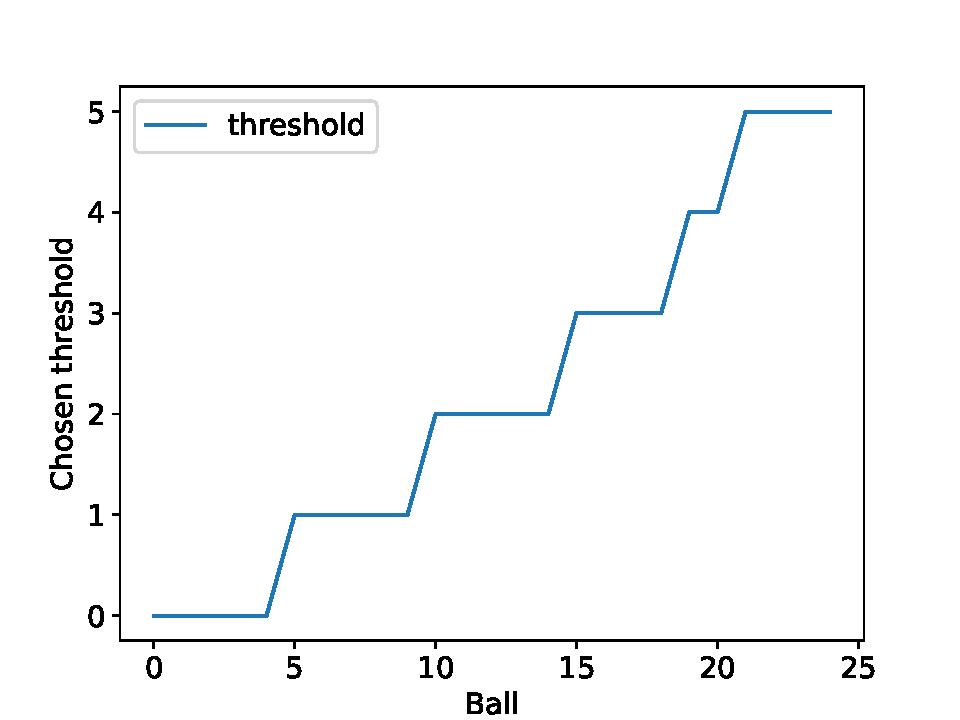
\includegraphics[scale=0.36]{Chapter4/Figs/dp_increasing_threshold_1.pdf}
\end{minipage}\hfill
\begin{minipage}[t]{.32\linewidth}
  \centering
  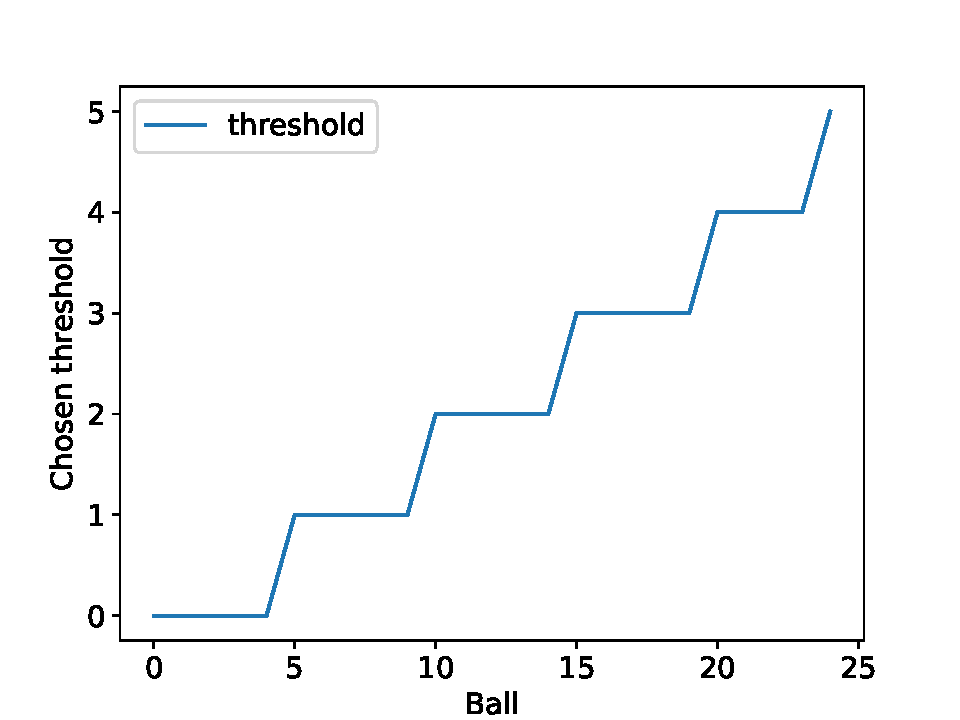
\includegraphics[scale=0.36]{Chapter4/Figs/dp_increasing_threshold_2.pdf}
\end{minipage}\hfill
\begin{minipage}[t]{.32\linewidth}
  \centering
  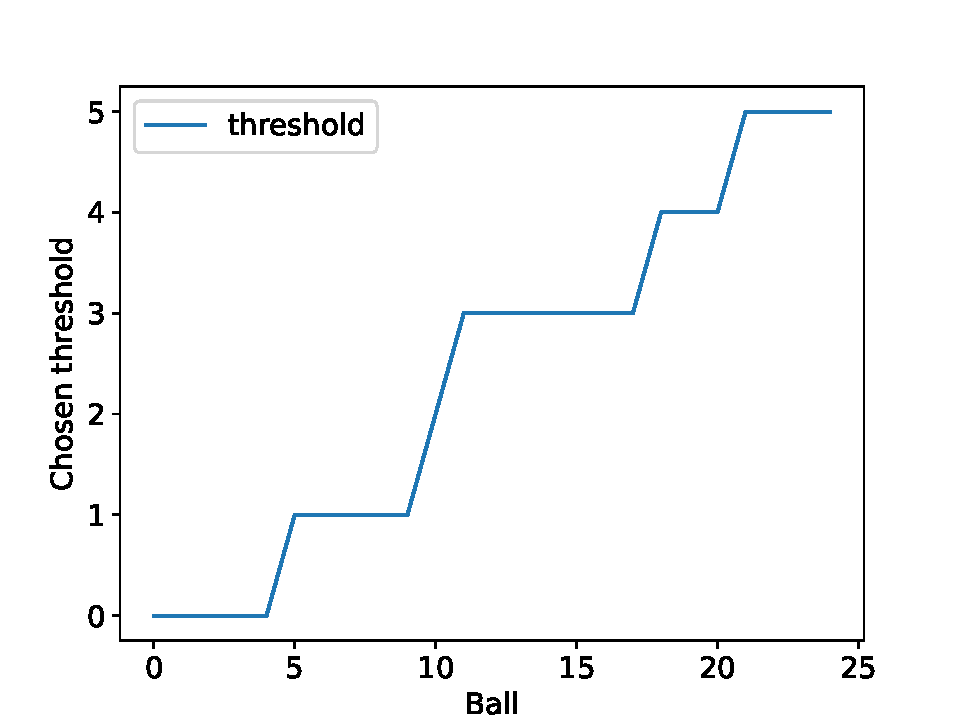
\includegraphics[scale=0.36]{Chapter4/Figs/dp_increasing_threshold_3.pdf}
\end{minipage}
\caption{Runs of the \DP strategy for $n=5$, $m=25$ showing the increasing threshold property. Note that the actual load vectors are not displayed.}
\label{dp-increasing-threshold}
\end{figure}



\NOTE{D}{This would be part of a ``thorough'' qualitative evaluation. If would spot a trend it would also be nice to support it with some quantitative data. Andor: do you still think I should add it or I have convinced you that we should rather remove things not add?}
This is a very surprising conjecture, because the \Threshold strategy and other strategies for similar settings that have been shown to be asymptotically optimal do not have this property (this is not a contradiction as they are only optimal up to a constant factor), they are mostly not even slicing strategies.


\begin{remark}
Conjecture~\ref{conjecture: two-thinning-increasing-threshold} has been verified by showing that this property holds for the (optimal) \DP strategy for several combinations of $n$ and $m$. 
\end{remark}


To get a deeper understanding of the optimal (\DP) strategy, using an auxiliary DP algorithm, I analysed the probabilities of it reaching different states (sorted load vectors) during an execution (see Figure~\ref{two-thinning-dp-state-distribution}). The main conclusions are:

\begin{itemize}
    \item There is a big gap between the probabilities of reaching different states by the optimal strategy. For example, the most likely final state $(0, 0, 0, 0, 0, 0, 1, 1, 1, 1, 1, 1, 1, 1, 2, 2, 2, 2, 2, 2)$ has a probability of almost a quarter, which is very large among $627$ possible final states. \NOTE{A}{Break lines for long math syntax.}
    \item The entropy of the probabilities of the final states is $\approx 3.36$ bits, which is nearly a third of the entropy of a uniform distribution with the same number of states.
    \item In future work, the presence of many small probability states could be exploited to optimise the training of RL algorithms, e.g.\ finding the most relevant curriculum for curriculum learning.
    \item The naive simulation of any strategy uses $m\cdot \log_2 n=20\cdot \log_2 20\approx 86$ bits for $n=m=20$, so the $86-3.36\approx 83$ bits gap highlights that naive simulation is very inefficient.
\end{itemize}

\NOTE{T}{I think you may get a similar distribution if you do the following experiment. You sample $n$ times, independently from a normal distribution $N(0,\sigma)$. A few combinations, e.g., $(0,\ldots,0)$ have the highest probability, but most combinations are like $(\pm \sigma,\pm \sigma)$ etc, which may correspond to your peak around $-50$. Andor: interesting -- is there any way that I could mention it in a reasonable way?}

In many real-world applications it does not suffice if the maximum load is low in expectation, it should also be small with high probability. As demonstrated in Figure~\ref{two-thinning-dp-maxload-distribution}, the \DP strategy has this property (agreeing with most of the strategies/protocols in the balls-into-bins literature).

\begin{figure}
\centering
\begin{minipage}[t]{.48\linewidth}
  \centering
  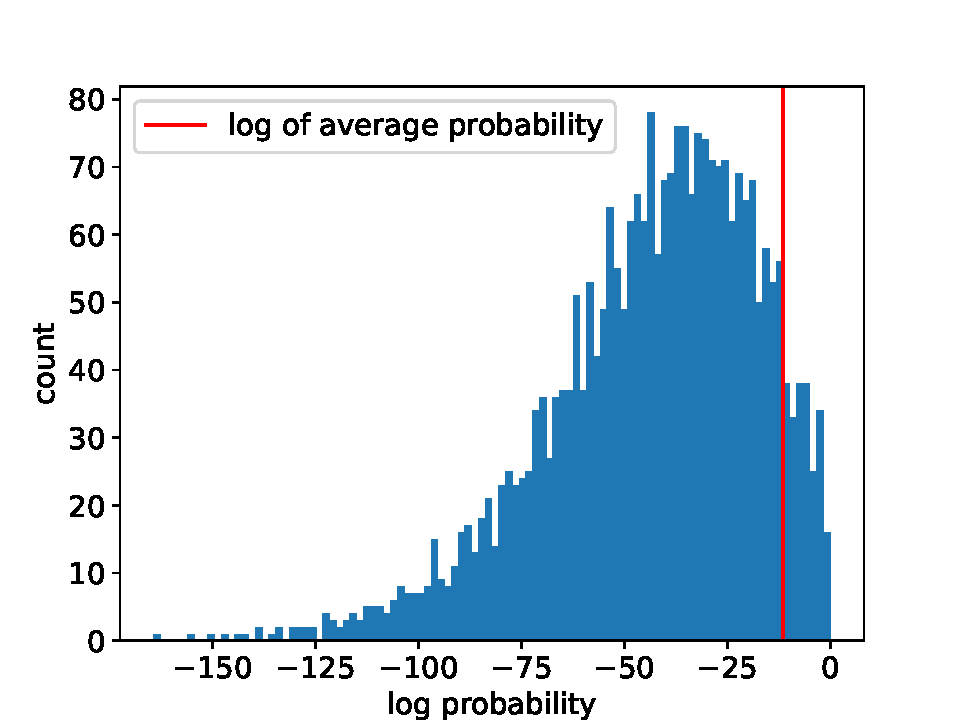
\includegraphics[scale=0.5]{Chapter4/Figs/state_distribution_20_20_all_log_count.pdf}
  \caption{The distribution of the probabilities of all the states for $n=m=20$, using the \DP strategy. Due to the skewness of the distribution, the values are shown on a log-scale.}
  \label{two-thinning-dp-state-distribution}
\end{minipage}\hfill
\begin{minipage}[t]{.48\linewidth}
  \centering
  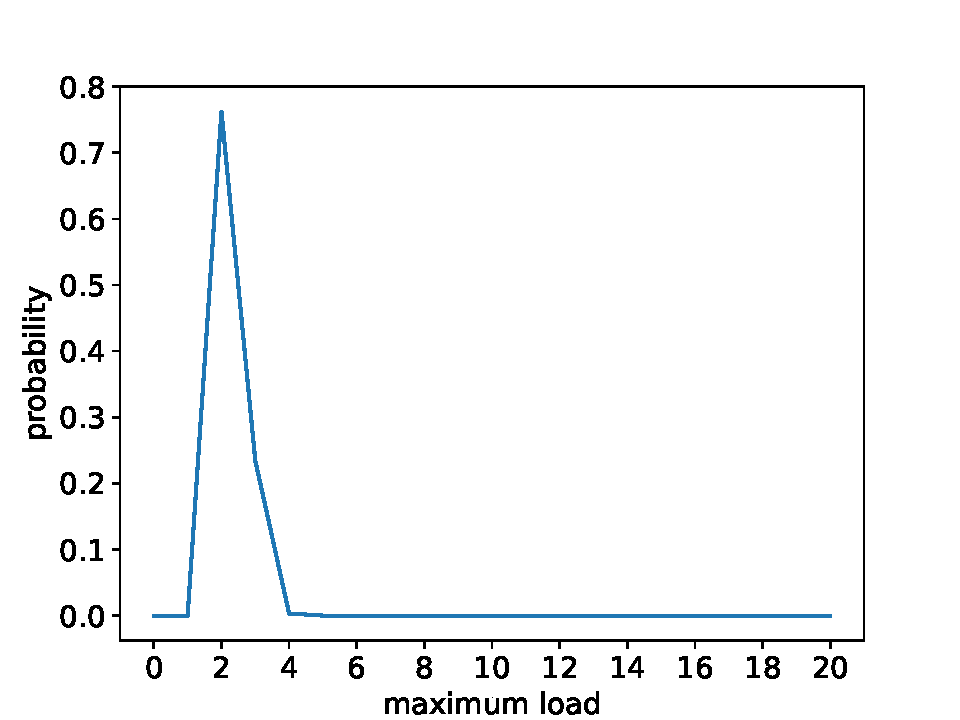
\includegraphics[scale=0.5]{Chapter4/Figs/max_load_distribution_20_20.pdf}
  \caption{The distribution of the final maximum loads for $n=m=20$, using the \DP strategy.}
  \label{two-thinning-dp-maxload-distribution}
\end{minipage}
\end{figure}


\subsection{Deep Q-Learning Analysis}


\subsubsection{Hyperparameter Analysis}


The Weights and Biases tool~\cite{biewald2020wandb} provides hyperparameter importance analysis. It calculates the correlation coefficient between the hyperparameters and the score, for each hyperparameter (green is positive, red is negative). To capture interactions between hyperparameters and also non-linear relationships, it additionally provides an importance score which is calculated based on Random Forests~\cite{biewald2020wandb}. Table~\ref{two-thinning-hyperparameter-importance} -- which is based on the tool -- shows the top $5$ hyperparameters based on the importance score.


We can observe that for \TwoThinning the most important hyperparameter is to use the normalised domain, which was discussed in Section~\ref{normalised-domain}. Also, limiting the maximum threshold that the agent can use efficiently restricts the search space, as discussed in Section~\ref{dqn-implmentation-two-thinning}. As can be seen in Appendix~\ref{hyperparameters}, the ideal maximum threshold is in fact around the target expected maximum load we want to achieve (which can be estimated in general based on theoretical results).



\newcommand{\Progress}[2]{
\begin{tikzpicture}
\draw[fill=#2!10!white] (0,0) rectangle (5, 0.3);
\draw[fill=#2!50!white] (0,0) rectangle (5 * #1, 0.3);
\end{tikzpicture}
}

\begin{table}
\begin{center}
\begin{tabular}{lcc}
 \textbf{Hyperparameter} & \textbf{Importance} & \textbf{Correlation} \\
 \addlinespace[0.2cm]
 \texttt{use\_normalised} & \Progress{0.362}{blue} & \Progress{0.602}{green} \\
 \texttt{max\_threshold} & \Progress{0.141}{blue} & \Progress{0.496}{red} \\
 \texttt{num\_rnn\_layers} & \Progress{0.07}{blue} & \Progress{0.239}{green} \\
 \texttt{rnn\_hidden\_size} & \Progress{0.069}{blue} & \Progress{0.166}{green} \\
 \texttt{pre\_train\_episodes} & \Progress{0.06}{blue} & \Progress{0.103}{red} \\
\end{tabular}
\caption{\TwoThinning hyperparameter importance~\cite{biewald2020wandb} for $n=20$, $m=400$.}
\label{two-thinning-hyperparameter-importance}
\end{center}
\end{table}




\subsubsection{Training}


\begin{figure}[h]
    \centering
    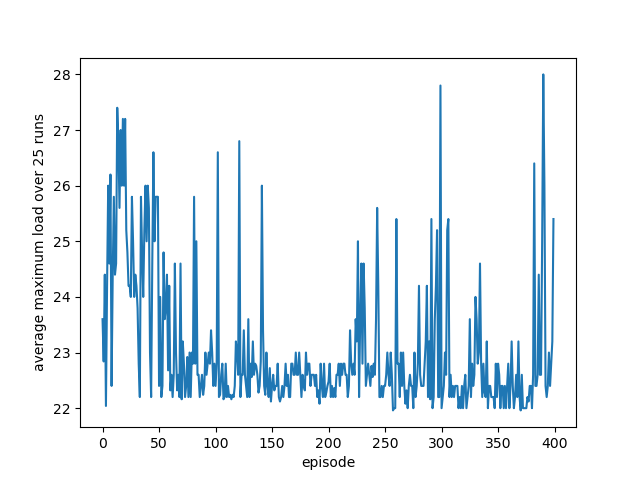
\includegraphics[scale=0.6]{Chapter4/Figs/training_progression_20_400.png}
    \caption{\TwoThinning training curve for $n=20$, $m=400$}
     \label{two-thinning-training-curve}
\end{figure}
\NOTE{T}{Maybe if you do some averaging to the plot, one could see a bit more the learning progress. For example, you could take the average maximum load over the first $x$ episodes.}\NOTE{A}{Change png to pdf!}

As shown in Figure~\ref{two-thinning-training-curve}, improvement during training decays very quickly, and the agent is close to its best already at the start. This is again due to the normalised load domain outlined above -- I checked the training curve without the normalised load domain trick as well, and that shows a much more usual training progression, though leading to a worse optimum. The oscillations in the training curve are mostly due to the inherent randomness in evaluation.


Motivated by the fact that in the normalised domain, a constant $0$ threshold is the \MeanThinning strategy, in Figure~\ref{two-thinning-constant-offset} I tried to see if this simple \MeanThinning strategy could be improved by choosing another constant ``offset'', not $0$. For $n=50$, $m=2500$, the best offset is $1$, and it achieves on average a final maximum load of $52.5$, which is very close to the the theoretical minimum $\frac{m}{n}=50$, and also beats the \DQN strategy. It holds for general $n$ and $m$ that the best offset is usually slightly above $0$.

\begin{figure}[h]
    \centering
    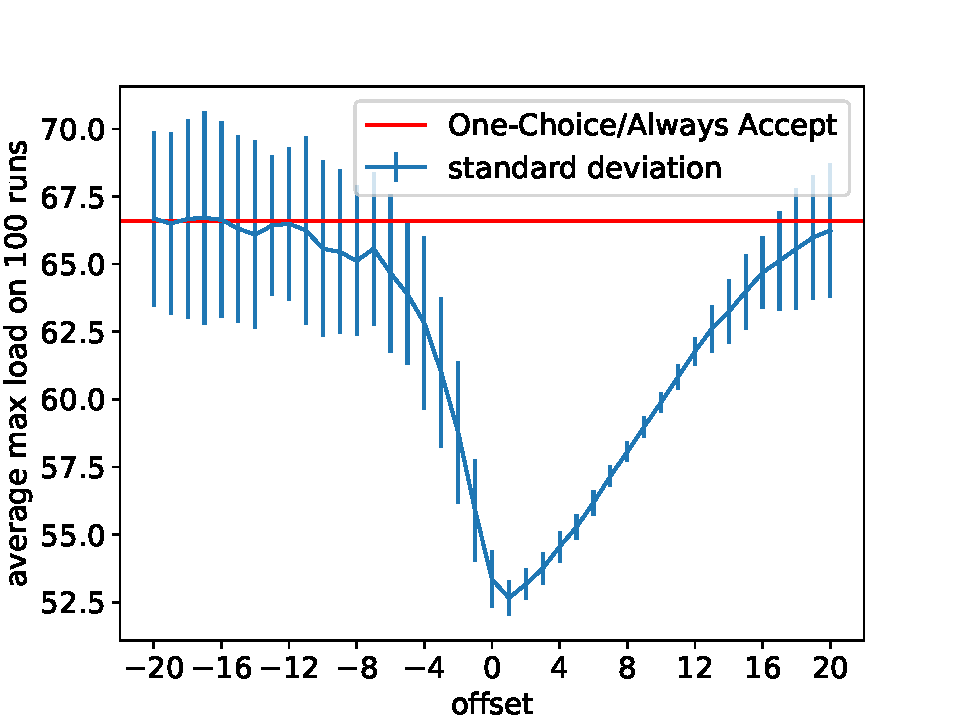
\includegraphics[scale=0.6]{Chapter4/Figs/offset_analysis_50_2500.pdf}
    \caption{Comparing \ConstantOffset strategies for $n=50$, $m=2500$.}
    \label{two-thinning-constant-offset}
\end{figure}


\NOTE{T}{Another interesting ``philosophical'' insight from the figure seems to be that having a too small offset is more detrimental than having a too large offset.}

\NOTE{D}{!!Can you also try $n = 10^4$ and $m = 10^6$ (or larger)?}


The Deep-Q Learning algorithm -- which is as shown above, statistically significantly better than Mean-Thinning -- in fact often learns a strategy similar to a \ConstantOffset strategy, as can be seen in Figure \ref{two-thinning-dqn-thresholds}. The short sporadic ``jumps'' are very challenging for the agent to get rid of, due to the reasons outlined in Section~\ref{two-thinning-comparison}. To avoid this, future work could constrain the agent to change (and only increase) the threshold by at most $1$ after each ball, which is motivated by Conjecture~\ref{conjecture: two-thinning-smooth-threshold}.


\begin{conjecture}\label{conjecture: two-thinning-smooth-threshold}
There exists an optimal (slicing) strategy such that its chosen thresholds are changed by at most $1$ in any step during an execution.
\end{conjecture}


\begin{remark}
Together with Conjecture~\ref{conjecture: two-thinning-increasing-threshold} these would imply an optimal strategy whose threshold either stays the same or increases by $1$ in each step.
\end{remark}


\begin{figure}[h]
    \centering
    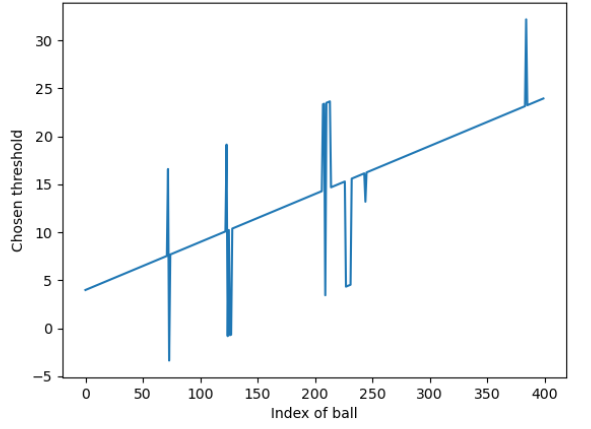
\includegraphics[scale=0.6]{Chapter4/Figs/dqn_learnt_thresholds.png}
    \caption{Analysis of the chosen thresholds of the \DQN strategy for a run of $n=20$, $m=400$.}
    \label{two-thinning-dqn-thresholds}
\end{figure}



\section{\KThinning}



\subsection{Comparison of Strategies}


Since the drawback (TLE) of the \DP strategy has already been highlighted for \TwoThinning, I decided to focus on smaller cases here where a full comparison is feasible and highlight other patterns related to the choice of $k$.


\begin{table}[h!]
\centering
\resizebox{\textwidth}{!}{%
\begin{tabular}{|l|c|c|c|c|c|c|c|c|}
\hline
                                & \multicolumn{4}{c|}{$n=5$} & \multicolumn{4}{c|}{$n=25$}\\ \hline
                                & \multicolumn{4}{c|}{$m=20$} & \multicolumn{4}{c|}{$m=50$}\\ \hline
Strategy                                & $k=2$ & $k=3$ & $k=5$ & $k=10$ & $k=2$ & $k=3$ & $k=5$ & $k=10$ \\ \hline
\AlwaysAccept & 7.73 $\pm$ 0.11 & 7.76 $\pm$ 0.11 & 7.59 $\pm$ 0.11 & 7.67 $\pm$ 0.11 & 5.82 $\pm$ 0.09 & 5.79 $\pm$ 0.08 & 5.83 $\pm$ 0.09 & 5.86 $\pm$ 0.09 \\ \hline \LocalRewardOptimiser & \textbf{6.09 $\pm$ 0.05} & 5.74 $\pm$ 0.04 & 5.41 $\pm$ 0.04 & 5.13 $\pm$ 0.03 & 4.17 $\pm$ 0.04 & 3.73 $\pm$ 0.04 & 3.20 $\pm$ 0.04 & 3.00 $\pm$ 0.01 \\ \hline \Quantile & 6.23 $\pm$ 0.05 & 5.99 $\pm$ 0.04 & 5.58 $\pm$ 0.04 & 5.17 $\pm$ 0.03 & 4.36 $\pm$ 0.06 & 3.66 $\pm$ 0.05 & 3.12 $\pm$ 0.03 & \textbf{3.00 $\pm$ 0.00} \\ \hline \DP & 6.13 $\pm$ 0.05 & \textbf{5.73 $\pm$ 0.04} & \textbf{5.39 $\pm$ 0.04} & \textbf{5.11 $\pm$ 0.03} & \textbf{4.08 $\pm$ 0.04} & \textbf{3.63 $\pm$ 0.04} & \textbf{3.10 $\pm$ 0.03} & \textbf{3.00 $\pm$ 0.00} \\ \hline \Threshold & 6.56 $\pm$ 0.06 & 6.29 $\pm$ 0.05 & 6.14 $\pm$ 0.04 & 5.92 $\pm$ 0.03 & 4.53 $\pm$ 0.05 & 4.19 $\pm$ 0.04 & 3.92 $\pm$ 0.03 & 3.96 $\pm$ 0.03 \\ \hline \DQN & 6.67 $\pm$ 0.07 & 5.87 $\pm$ 0.05 & 5.60 $\pm$ 0.05 & 5.22 $\pm$ 0.04 & 4.51 $\pm$ 0.05 & 3.95 $\pm$ 0.05 & 3.42 $\pm$ 0.04 & 3.04 $\pm$ 0.02 \\ \hline 
\end{tabular}}

\caption{Average maximum load of \KThinning strategies with $95\%$ confidence intervals}
\label{tab:k-thinning-comparison}
\end{table}


Intuitively, the larger $k$ is, the better a strategy can do, and the table confirms it for most of the strategies. We can see from the table that the \Quantile and \LocalRewardOptimiser strategies are almost as good as the \DP strategy for most values of $n$, $m$ and $k$, even though neither of those strategies consider future rewards. For large $k$ ($5$ or $10$) and not too large $n$, strategies can control with high probability where to place the ball. Nevertheless, this kind of advantage is much easier to exploit by a manual algorithm, than to learn by Deep Q-Learning.



\subsection{Theoretical Analysis}


In Figure~\ref{k-thinning-dp-maxload} we can see how the value of $k$ influences the (optimal) DP Strategy. While there is a large improvement from $k=2$ to $k=3$ (e.g. the probability of $\mathrm{maxload}=6$ becomes negligible), we can observe diminishing returns by further increasing $k$.


\begin{figure}[h]
    \centering
    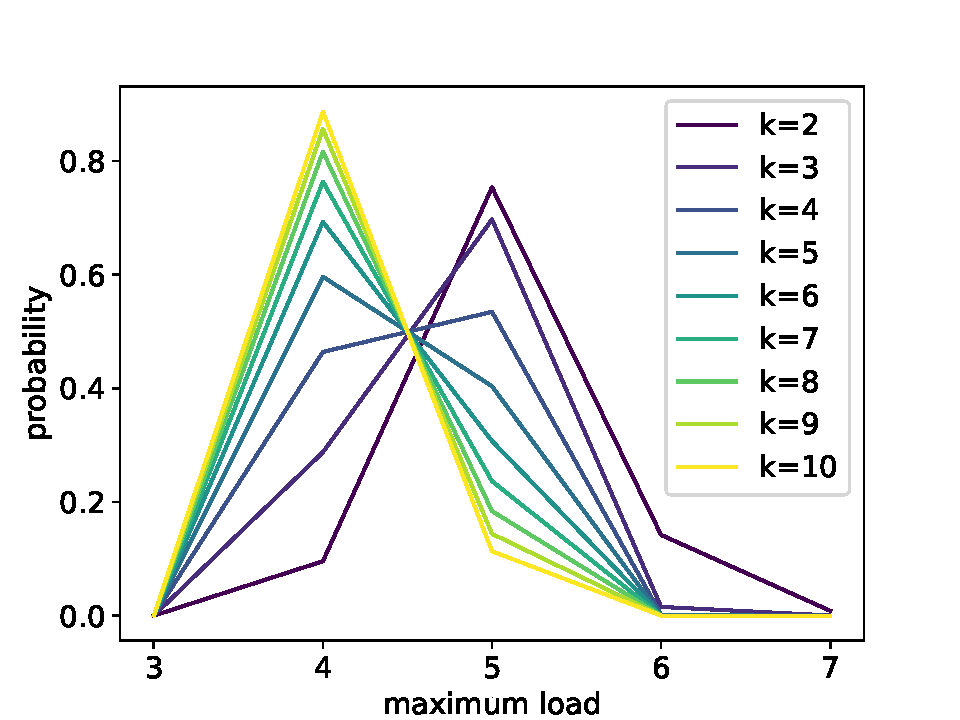
\includegraphics[scale=0.6]{Chapter4/Figs/k_thinning_max_load_distribution_5_20.pdf}
    \caption{Analysis of the final maximum load distribution of the DP strategy for $n=20$, $m=400$ and different values of $k$.}
    \label{k-thinning-dp-maxload}
\end{figure}
\NOTE{T}{Better to use some color scheme (red to green) when transitioning from $k=2$ to $k=10$}

Now I present a lemma about optimal strategies:
\begin{lemma} \label{lemma: k-thinning-increasing-threshold}
There exists an optimal strategy, such that if it accepts a bin with $x$ choices left, it would accept the same bin (with the same loads) with $y<x$ choices left as well. In other words, an optimal strategy should never become more selective after rejecting some options.
\end{lemma}


\begin{proof}
    The proof is similar in structure to the proof of Lemma~\ref{lemma: thresholdproperty}.
\end{proof}

\begin{remark}
Lemma~\ref{lemma: k-thinning-increasing-threshold} has been verified by showing that this property holds for the (optimal) \DP strategy for several combinations of $n$, $m$ and $k$. Also note that Conjecture ~\ref{conjecture: two-thinning-increasing-threshold} generalises to \KThinning as well, and it has been verified similarly.
\end{remark}


\subsection{Deep Q-Learning Analysis}



\subsubsection{Hyperparameter Analysis}



\begin{table}
\begin{center}
\begin{tabular}{lcc}
 \textbf{Hyperparameter} & \textbf{Importance} & \textbf{Correlation} \\
 \addlinespace[0.2cm]
 \texttt{optimise\_freq} & \Progress{0.138}{blue} & \Progress{0.42}{red} \\
 \texttt{target\_update\_freq} & \Progress{0.133}{blue} & \Progress{0.124}{green} \\
 \texttt{eps\_decay} & \Progress{0.088}{blue} & \Progress{0.051}{red} \\
 \texttt{pre\_train\_episodes} & \Progress{0.084}{blue} & \Progress{0.293}{green} \\
 \texttt{batch\_size} & \Progress{0.074}{blue} & \Progress{0.205}{red} \\
\end{tabular}
\caption{\KThinning hyperparameter importance~\cite{biewald2020wandb} for $n=20$, $m=400$.}
\label{k-thinning-hyperparameter-analysis}
\end{center}
\end{table}


We can observe in Table~\ref{k-thinning-hyperparameter-analysis} that the normalised load domain trick is not as crucial for \KThinning as it was for \TwoThinning\NOTE{A}{Mention some bullshit possible reason?}. On the other hand, the analysis suggests more frequent optimisation update steps and more curriculum learning (pretraining) episodes. 


\subsubsection{Training}


\begin{figure}[h]
    \centering
    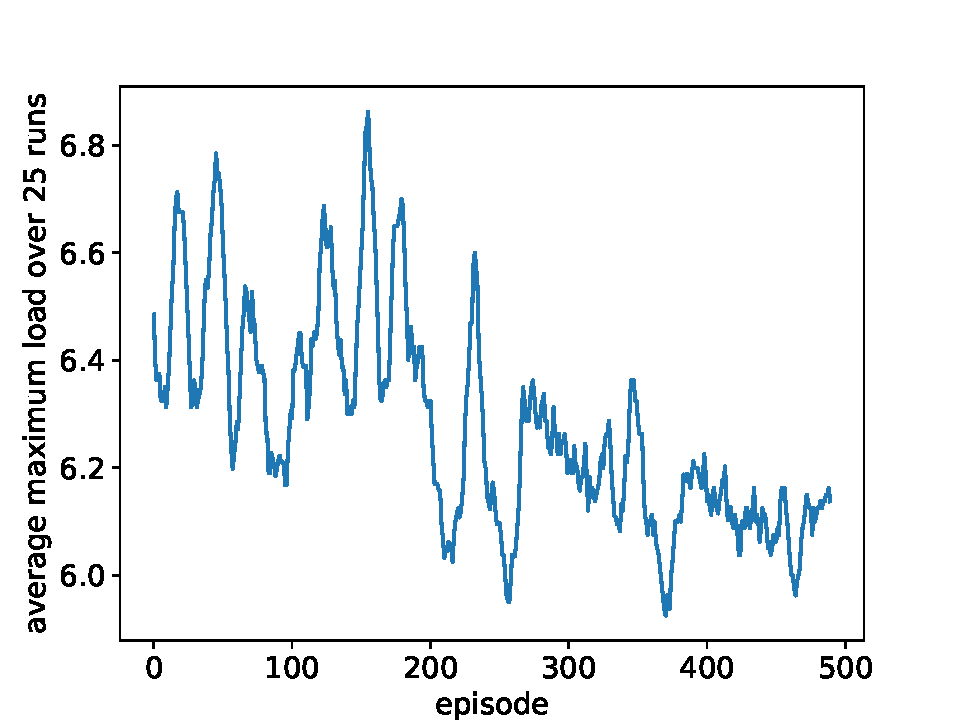
\includegraphics[scale=0.6]{Chapter4/Figs/training_progression_rolling_window_5_25_3.pdf}
    \caption{\KThinning training curve for $n=5$, $m=25$, $k=3$, with $10$ episodes wide rolling window averaging for readability purposes.}
    \label{k-thinning-training-curve}
\end{figure}


The training progression shown in Figure~\ref{k-thinning-training-curve} is similar to \TwoThinning, so I do not discuss it any further.


\section{\GraphicalTwoChoice}


\subsection{Comparison of Strategies}
\begin{table}[h!]
\centering
\resizebox{\textwidth}{!}{%
\begin{tabular}{|l|c|c|c|c|c|c|c|c|c|}
\hline
                                & \multicolumn{3}{c|}{$n=4$} & \multicolumn{3}{c|}{$n=16$} & \multicolumn{3}{c|}{$n=32$}\\ \hline
                                & \multicolumn{3}{c|}{$m=25$} & \multicolumn{3}{c|}{$m=50$} & \multicolumn{3}{c|}{$m=32$}\\ \hline
Strategy                                & Cycle & Hypercube & Complete & Cycle & Hypercube & Complete & Cycle & Hypercube & Complete \\ \hline
\Greedy & 7.06 $\pm$ 0.02 & 7.06 $\pm$ 0.02 & 7.19 $\pm$ 0.04 & \textbf{4.75 $\pm$ 0.05} & \textbf{4.51 $\pm$ 0.05} & \textbf{4.40 $\pm$ 0.05} & \textbf{2.40 $\pm$ 0.05} & \textbf{2.33 $\pm$ 0.04} & \textbf{2.26 $\pm$ 0.04} \\ \hline \Random & 8.96 $\pm$ 0.12 & 8.97 $\pm$ 0.12 & 8.84 $\pm$ 0.11 & 6.49 $\pm$ 0.09 & 6.62 $\pm$ 0.10 & 6.69 $\pm$ 0.10 & 3.49 $\pm$ 0.06 & 3.52 $\pm$ 0.07 & 3.50 $\pm$ 0.06 \\ \hline \LocalRewardOptimiser & 7.12 $\pm$ 0.03 & 7.11 $\pm$ 0.03 & 7.25 $\pm$ 0.04 & 4.87 $\pm$ 0.06 & 4.77 $\pm$ 0.05 & 4.74 $\pm$ 0.05 & 2.53 $\pm$ 0.05 & 2.44 $\pm$ 0.04 & 2.38 $\pm$ 0.04 \\ \hline \DP & \textbf{7.04 $\pm$ 0.02} & \textbf{7.03 $\pm$ 0.01} & \textbf{7.17 $\pm$ 0.03} & TLE & TLE & TLE & TLE & TLE & TLE \\ \hline \DQN & 7.11 $\pm$ 0.03 & 7.11 $\pm$ 0.03 & 7.31 $\pm$ 0.05 & 4.88 $\pm$ 0.07 & 4.53 $\pm$ 0.05 & 4.50 $\pm$ 0.05 & 2.68 $\pm$ 0.06 & 2.54 $\pm$ 0.05 & 2.60 $\pm$ 0.06 \\ \hline 
\end{tabular}}

\caption{Average maximum load of \GraphicalTwoChoice strategies with $95\%$ confidence intervals\protect\footnotemark}
\label{tab:graphical-two-choice-comparison}
\end{table}

\footnotetext{Note that for $n=4$, the \CycleGraph and the \HypercubeGraph are the same.}

The most important conclusions from Table~\ref{tab:graphical-two-choice-comparison} are:

\begin{itemize}
    \item The \Greedy strategy is not exactly optimal, as can be seen from the $n=4$ case (I will provide an explicit counterexample in Lemma~\ref{lemma: greedy-suboptimal}). On the other hand, it is close to the performance of the \DP strategy, and when that is not applicable, \Greedy is by far the best.
    \item While for larger $n$, agreeing with the intuition the \CompleteGraph is the most favourable for \Greedy, it works better on the \CycleGraph for $n=4$. 
    \item The \DQN strategy performs performs consistently, but it cannot always exploit the subtle suboptimalities of \Greedy. Its performance is comparable to the performance of the \LocalRewardOptimiser strategy.
    
\end{itemize}


\subsection{Theoretical Analysis}

First I prove the most surprising result of this section.

\begin{lemma} \label{lemma: greedy-suboptimal}
There exists a graph, such that the \Greedy strategy is suboptimal with respect to the expected final maximum load of \GraphicalTwoChoice.
\end{lemma}

\begin{proof}
Using the \DP strategy for the \CycleGraph with $n=4$ bins $m=6$ balls, I found a state $s$ (i.e.\ a load vector $v$ and edge $e$), where choosing the less loaded bin is suboptimal. Denoting the nodes as ($1$-based) indices in the load vector, the counterexample state is $v=(0,1,0,2)$,  $e=(2,3)$ i.e.\ there is an edge between the second and third bin. \Greedy would choose the third bin, but if all the later edges are $(3,4)$, $\mathrm{maxload}>2$ cannot be avoided (see Figure~\ref{greedy-counterexample}). On the other hand, by choosing the second bin and then picking the odd-indexed endpoints of the later edges, the maximum load will always be $2$. Therefore, the expected final maximum load of choosing the second bin (and then playing optimally) is $2.0$, while that of choosing the third bin is between $2.0$ and $3.0$.
\end{proof}



\begin{figure}
    \centering
    \begin{tikzpicture}
    \Tree [.$(0,\underline{\mathbf{1}},\underline{\mathbf{0}},2)$
    [.$(0,1,\underline{\mathbf{1}},\underline{\mathbf{2}})$
    [.$(0,1,\underline{\mathbf{2}},\underline{\mathbf{2}})$
    [.$(0,1,3,2)$ ] $\ldots$ ] $\ldots$ ]
    [.$(0,2,0,2)$ $\ldots$ ]]
    \end{tikzpicture}
    \caption{Counterexample for the optimality of \Greedy, showing that choosing the second bin can lead to a maximum load of $3$ while choosing the third bin cannot.}
    \label{greedy-counterexample}
\end{figure}



To better understand the impact of the graph structure on \Greedy, I analysed the relationship between the degree $d$ of the graph and how well \Greedy performs on it. I created $1000$ random regular graphs for each degree $1\leq d \leq 31$ of the $n=m=32$ case. \NOTE{T}{Very interesting... I would have hoped that maybe for $d \approx 15$ or so you would get the best performance, which in a way, would generalise the cycle for small values of $n$. Andor: Interesting idea, I don't know how to generalise the cycle for smalle values of $n$.} We can see in Figure~\ref{greedy-random-regular-analysis} that smaller degrees hurt \Greedy, but after around $d=20$, the performance no longer improves.


\begin{figure}[h]
    \centering
    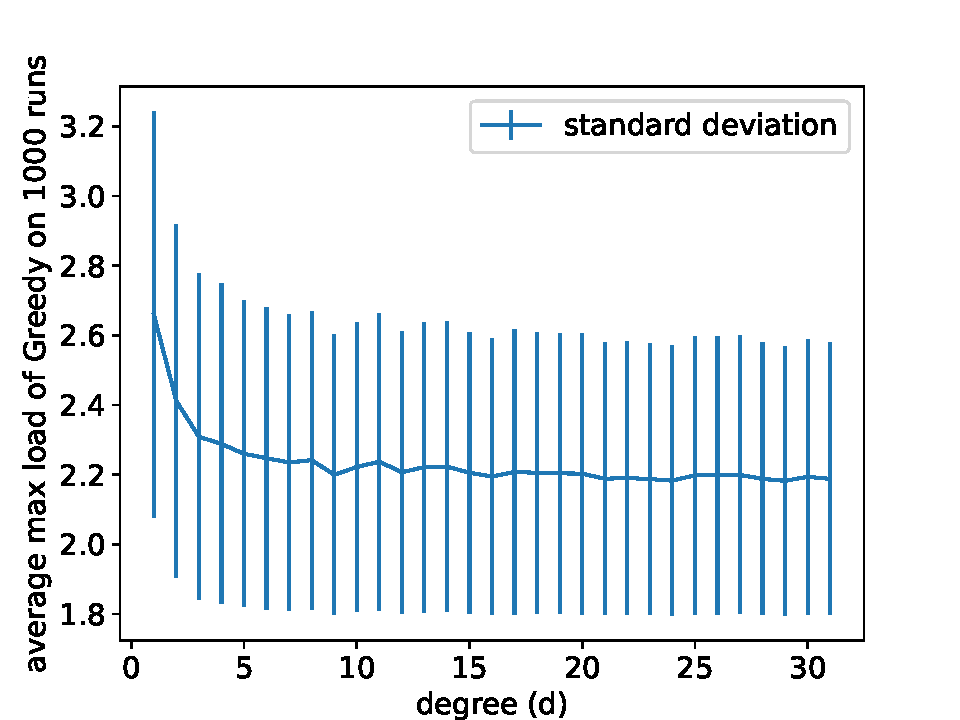
\includegraphics[scale=0.6]{Chapter4/Figs/greedy_degree_analysis_32_32.pdf}
    \caption{Relating the degree of the graph to the performance of Greedy for $n=m=32$.}
    \label{greedy-random-regular-analysis}
\end{figure}


\subsection{Deep Q-Learning Analysis}

To better understand the difficulty in finding an optimal strategy, I extended the \CycleGraph counterexample from Lemma ~\ref{lemma: greedy-suboptimal} to load vectors of the form $(0, a, 0, b)$, with the next edge still going between the second and third bins. Figure~\ref{greedy-counterexample-analysed} and Figure~\ref{greedy-counterexample-analysed-for-dqn} show that the shape of the region containing counterexamples to the \Greedy strategy is difficult to characterise, and to precisely learn by RL. By using the $\Phi_{neigh}$ potential function for Deep Q-Learning, the agent is guided towards choosing second bin, and by using a graph-oblivious potential (e.g.\ $\Phi_{max}$), the agent is guided towards choosing the third bin. Therefore, neither of the potential functions is perfect. We can indeed see in Figure~\ref{greedy-counterexample-analysed-for-dqn} that the DQN could not learn the exact pattern, though there is some resemblance.


\begin{figure}
\centering
\begin{minipage}[t]{.48\linewidth}
  \centering
  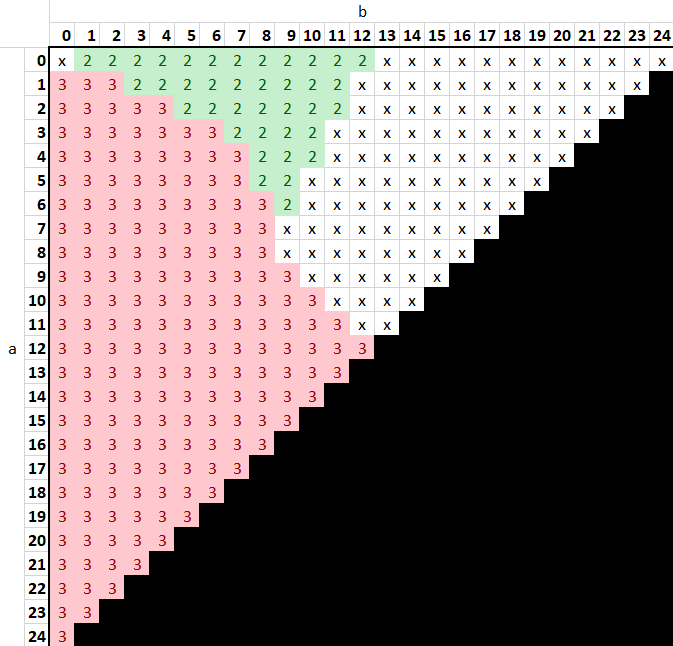
\includegraphics[scale=0.45]{Chapter4/Figs/0a0b_4_25_analysis.png}
  \caption{The optimal decisions for the \CycleGraph with $n=4$, $m=25$, load vector $(0,a,0,b)$ and edge $(2,3)$. Green indicates choosing the second bin is better, red indicates choosing the third bin is better, and $x$ indicates that they have the same expected score.}
  \label{greedy-counterexample-analysed}
\end{minipage}\hfill
\begin{minipage}[t]{.48\linewidth}
  \centering
  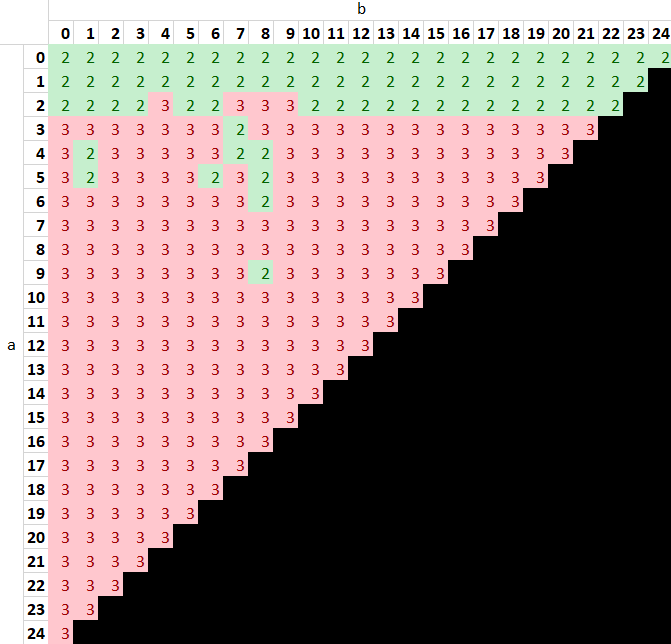
\includegraphics[scale=0.45]{Chapter4/Figs/0a0b_4_25_analysis_dqn.png}
  \caption{The decisions made by the \DQN strategy in the situation from Figure~\ref{greedy-counterexample-analysed}.}
  \label{greedy-counterexample-analysed-for-dqn}
\end{minipage}
\end{figure}



\subsubsection{Hyperparameter Analysis}


Analysing Table~\ref{graphical-two-choice-hyperparameter-importance}, the negative correlation of ``hidden\_size'' and ``num\_lin\_layers'' with the score suggests that adding more parameters to the DQN does not help. 


\begin{table}
\begin{center}
\begin{tabular}{lcc}
 \textbf{Hyperparameter} & \textbf{Importance} & \textbf{Correlation} \\
 \addlinespace[0.2cm]
 \texttt{pre\_train\_episodes} & \Progress{0.207}{blue} & \Progress{0.450}{green} \\
 \texttt{num\_lin\_layers} & \Progress{0.190}{blue} & \Progress{0.344}{red} \\
 \texttt{hidden\_size} & \Progress{0.162}{blue} & \Progress{0.462}{red} \\
 \texttt{optimise\_freq} & \Progress{0.074}{blue} & \Progress{0.333}{red} \\
 \texttt{target\_update\_freq} & \Progress{0.071}{blue} & \Progress{0.124}{red} \\
\end{tabular}
\caption{\GraphicalTwoChoice hyperparameter importance for the \CycleGraph with $n=4$ and $m=25$ \cite{biewald2020wandb}}
\label{graphical-two-choice-hyperparameter-importance}
\end{center}
\end{table}


\subsubsection{Training}

Figure~\ref{graphical-two-choice-training-curve} shows a much steadier improvement during training for \GraphicalTwoChoice than what we saw for \TwoThinning and \KThinning. This is mostly because there is no reasonable easy-to-learn initial strategy for \GraphicalTwoChoice with the chosen MDP formulation, unlike the \ConstantOffset strategies for \TwoThinning.

\begin{figure}[h] 
    \centering
    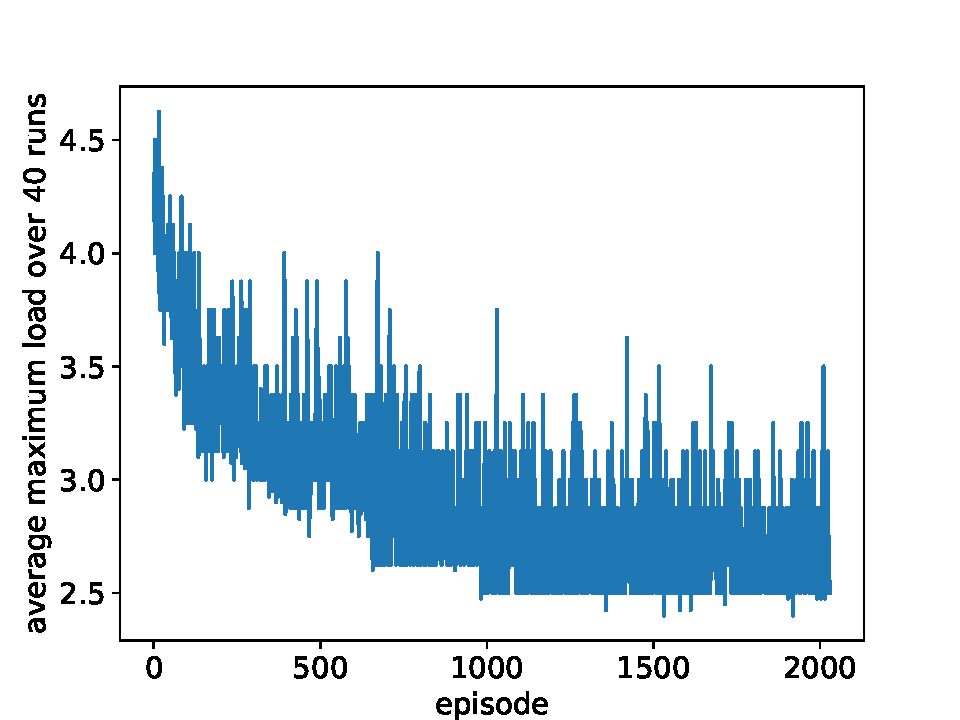
\includegraphics[scale=0.6]{Chapter4/Figs/training_progression_hypercube_32_32.pdf}
    \caption{\GraphicalTwoChoice training curve for the \CycleGraph with $n=m=32$.}
    \label{graphical-two-choice-training-curve}
\end{figure}


%!TEX root = ../thesis.tex

\chapter{Conclusions}\label{conclusion}

\ifpdf
    \graphicspath{{Chapter3/Figs/Raster/}{Chapter3/Figs/PDF/}{Chapter3/Figs/}}
\else
    \graphicspath{{Chapter3/Figs/Vector/}{Chapter3/Figs/}}
\fi



\section{Applicability of RL to Balls into Bins}
\NOTE{A}{Analysis of Balls into Bins using RL. The original title suggests that it is actually applicable.}

As we have seen for each of the three settings, the difference between good and bad decisions are very subtle, which make RL very challenging to apply. Even with all the tricks I tried, it couldn't consistently outperform simpler heuristic strategies, such as the Local Reward Optimiser Strategy. Also, in order to get acceptable results, extensive and precise hyperparameter tuning was necessary in most cases. \NOTE{A}{Write something positive as well?}



\section{Lessons Learnt}

I experienced the rich nature of RL, and I realised that it is a very complex field, which I would like to learn more about in the future. 

Even though the project was planned to focus more on RL, we also obtained several theoretical insights via analysing strategies. This required me to deeply understand the nature of balls into bins, about which I learnt a lot by background reading, and exchanging ideas with my expert supervisors. 

\section{Future Work}

Apart from the ideas mentioned in other chapters, it is definitely possible to try other ideas for improving RL, and hopefully get closer to the optimal strategies. For examples, Graph Neural Networks could be tried for the \textsc{Graphical Two-Choice} setting, or instead of Deep Q-Learning, other RL algortihms, such as Policy Gradients could be experimented with. 


Also, we left some open theoretical questions (conjectures), and by analysing the optimal (DP) strategies more closely, several other properties might be derived, that could even help the design of simple yet effective strategies.


On a more practical note, future work should consider extending and analysing the discussed settings into more realistic and more challenging ones, e.g. as discussed in Chapter \ref{introduction}, the servers would usually synchronize their loads less frequently. \NOTE{A}{Give another example?}
%\include{Chapter6/chapter6}
%\include{Chapter7/chapter7}



% ********************************** Back Matter *******************************
% Backmatter should be commented out, if you are using appendices after References
%\backmatter

% ********************************** Bibliography ******************************
\begin{spacing}{0.9}

% To use the conventional natbib style referencing
% Bibliography style previews: http://nodonn.tipido.net/bibstyle.php
% Reference styles: http://sites.stat.psu.edu/~surajit/present/bib.htm

\bibliographystyle{apalike}
%\bibliographystyle{authoryear}
%\bibliographystyle{unsrt} % Use for unsorted references  
%\bibliographystyle{plainnat} % use this to have URLs listed in References

\bibliography{References/references} % Path to your References.bib file

\cleardoublepage


% If you would like to use BibLaTeX for your references, pass `custombib' as
% an option in the document class. The location of 'reference.bib' should be
% specified in the preamble.tex file in the custombib section.
% Comment out the lines related to natbib above and uncomment the following line.

%\printbibliography[heading=bibintoc, title={References}]


\end{spacing}

% ********************************** Appendices ********************************

\begin{appendices} % Using appendices environment for more functunality

\chapter{Alternative RL Algorithms}\label{alternativeRL} 



\paragraph{Sarsa-Learning}

Sarsa Learning is very similar to Q-Learning, and it generalises to Deep Sarsa-Learning just as Q-Learning generalises to Deep Q-Learning. The difference is that unlike Q-Learning, which is an off-policy method, Sarsa is on-policy. This means that in its update equation:

\begin{equation} \label{eq:sarsa-learningUpdate}
Q(s_t,a_t) \longrightarrow Q(s_t,a_t) + \alpha[( r_t + Q(s_{t+1}, a')) - Q(s_t,a_t)]
\end{equation}

$a'$ is also sampled according to the $\epsilon$-greedy technique, and it is not chosen greedily to be the best estimate like in Q-Learning. Then, naturally, the next chosen action will be exactly $a'$.

Due to this difference, Sarsa is more stable during training, but also it converges more slowly as it is not directly learning the optimal (greedy) policy, but an $\epsilon$-greedy policy~\cite{sutton2018RLbook}. Hence, Sarsa is more suitable when performance during training matters, and bad decisions are penalised (e.g. a valuable robot gets broken), but this is not the case in our protocols.

\paragraph{Monte Carlo Methods}


While Q- and Sarsa-Learning update their estimates based on other estimates (from one step ahead), Monte Carlo methods only use actual rewards for the update. This way, initialisation of the estimates doesn't matter that much, so it is more robust. In particular, the update rule in a simple Monte Carlo method is

\begin{equation} \label{eq:monte-carloUpdate}
Q(s_t,a_t) \longrightarrow Q(s_t,a_t) + \alpha[G_t - Q(s_t,a_t)]
\end{equation}

The problem with this approach is slow training. The reason is partly that if any exploration action (the case with probability $\epsilon$) is taken after timestep $t$, then, $Q(s_t,a_t)$ cannot be updated, since the new estimate doesn't necessarily reflect the estimated optimal value. Overall, Monte Carlo methods are rarely used in practice but they can be combined with Q-Learning (see e.g. the recent~\cite{wang2018montecarloqlearning}), which is an option I do not consider any further.

\paragraph{Policy Gradient}

Policy gradient methods are in contrast with the methods outlined above because they do not learn state- or action-value functions, instead they directly learn an optimal (stochastic) policy. Briefly, these algorithms use (another) neural network that represents the policy, and therefore returns probabilities choosing a given action in a given state. This leads to using the outputs of the neural network directly while playing the games during training, not the $\epsilon$-greedy technique. An advantage of this method is that there is no sharp boundary between the currently best estimated action and the second best, unlike for $\epsilon$-greedy. \NOTE{A}{Maybe add an equation. The problem is that it is a bit out of nowhere without derivation, and the derivation is a bit long.}



From the several policy gradient related approaches, I implemented the so-called Actor-Critic method~\cite{grondman2012actorcritic} and it didn't provide superior results to Deep Q-Learning or Sarsa-Learning. As explained in~\cite{bhandari2019policygradientconvergence}, policy gradient methods might converge to a local maximum, not the global optimum policy, and they might requires more time to converge. Policy gradient methods are still an active area of research, and while their usecase in unknown environments with state aliasing (where a stochastic strategy is desired) is clear, they are not yet the most widely used in full-knowledge scenarios like ours (i.e.\ where the exact current state is known).
\chapter{Alternative RL Algorithms}\label{alternativeRL} 



\paragraph{Sarsa-Learning}

Sarsa Learning is very similar to Q-Learning, and it generalises to Deep Sarsa-Learning just as Q-Learning generalises to Deep Q-Learning. The difference is that unlike Q-Learning, which is an off-policy method, Sarsa is on-policy. This means that in its update equation:

\begin{equation} \label{eq:sarsa-learningUpdate}
Q(s_t,a_t) \longrightarrow Q(s_t,a_t) + \alpha[( r_t + Q(s_{t+1}, a')) - Q(s_t,a_t)]
\end{equation}

$a'$ is also sampled according to the $\epsilon$-greedy technique, and it is not chosen greedily to be the best estimate like in Q-Learning. Then, naturally, the next chosen action will be exactly $a'$.

Due to this difference, Sarsa is more stable during training, but also it converges more slowly as it is not directly learning the optimal (greedy) policy, but an $\epsilon$-greedy policy~\cite{sutton2018RLbook}. Hence, Sarsa is more suitable when performance during training matters, and bad decisions are penalised (e.g. a valuable robot gets broken), but this is not the case in our protocols.

\paragraph{Monte Carlo Methods}


While Q- and Sarsa-Learning update their estimates based on other estimates (from one step ahead), Monte Carlo methods only use actual rewards for the update. This way, initialisation of the estimates doesn't matter that much, so it is more robust. In particular, the update rule in a simple Monte Carlo method is

\begin{equation} \label{eq:monte-carloUpdate}
Q(s_t,a_t) \longrightarrow Q(s_t,a_t) + \alpha[G_t - Q(s_t,a_t)]
\end{equation}

The problem with this approach is slow training. The reason is partly that if any exploration action (the case with probability $\epsilon$) is taken after timestep $t$, then, $Q(s_t,a_t)$ cannot be updated, since the new estimate doesn't necessarily reflect the estimated optimal value. Overall, Monte Carlo methods are rarely used in practice but they can be combined with Q-Learning (see e.g. the recent~\cite{wang2018montecarloqlearning}), which is an option I do not consider any further.

\paragraph{Policy Gradient}

Policy gradient methods are in contrast with the methods outlined above because they do not learn state- or action-value functions, instead they directly learn an optimal (stochastic) policy. Briefly, these algorithms use (another) neural network that represents the policy, and therefore returns probabilities choosing a given action in a given state. This leads to using the outputs of the neural network directly while playing the games during training, not the $\epsilon$-greedy technique. An advantage of this method is that there is no sharp boundary between the currently best estimated action and the second best, unlike for $\epsilon$-greedy. \NOTE{A}{Maybe add an equation. The problem is that it is a bit out of nowhere without derivation, and the derivation is a bit long.}



From the several policy gradient related approaches, I implemented the so-called Actor-Critic method~\cite{grondman2012actorcritic} and it didn't provide superior results to Deep Q-Learning or Sarsa-Learning. As explained in~\cite{bhandari2019policygradientconvergence}, policy gradient methods might converge to a local maximum, not the global optimum policy, and they might requires more time to converge. Policy gradient methods are still an active area of research, and while their usecase in unknown environments with state aliasing (where a stochastic strategy is desired) is clear, they are not yet the most widely used in full-knowledge scenarios like ours (i.e.\ where the exact current state is known).
%!TEX root = ../thesis.tex

\chapter{Hyperparameters}\label{hyperparameters} 


\section{List of Hyperparameters}


\NOTE{A}{Reorder in a more systematic way?}
\NOTE{A}{TODO: add usual values and/or reasons?}
\NOTE{A}{Should I add the ranges and options I used during the hyperparamter search?}
\begin{itemize} 
    \item batch size: the number of samples to take from the experience replay buffer using which the DQN is updated.
    
    \item $\epsilon$-start: for the $\epsilon$-greedy technique, it is common practice to gradually decrease $\epsilon$ during training. The reason is that after some training, less exploration is needed, as the best actions already start to take shape. I decrease $\epsilon$ according a negative exponential function, starting from $\epsilon$-start.
    
    \item $\epsilon$-decay: the decay parameter of the negative exponential function.\NOTE{T}{maybe better to use some formulas here?}
    
    \item $\epsilon$-end: as training goes on, $\epsilon$ converges to $\epsilon$-end.
     
    
    \item target update frequency: after every how many episodes is the target network synchronised with the main network.
    
    \item optimising frequency: this controls after every how many steps (i.e.\ actions) is the main network updated. Not updating it after every step is both a speed-up, and can control the reuse of samples in the experience replay buffer.
    
    \item memory capacity: the maximum size of the experience replay buffer.
    
    \item evaluation runs during training: to determine if the current model is better than the best one so far, I run this many full executions of the game with the current model, and average the scores. Note that this is very costly, as one execution of the game is equivalent to a full episode of training.
    
    \item maximum threshold of DQN: as mentioned in Section ~\ref{DQN}, the DQN is restricted to using only thresholds below this limit. A reasonable choice of this maximum threshold is around the target expected maximum load we expect to get, which can be estimated e.g.\ by the performance of simpler protocols, such as \OneChoice or \TwoChoice, or by theoretical results.
    
    \item loss function: the loss function to use between the current Q-value estimate and the new (``target'') Q-value estimate. \NOTE{A}{Explain better.}
    
    \item optimiser: the optimiser used for updating the neural network. \NOTE{A}{Update my code to include this as well.}
    
    \item learning rate: the learning rate of the optimiser. \NOTE{A}{Maybe I should also allow choosing other optimisers, such as simple SGD?}
    
    \item DQN -- hidden state size of RNN: this is the determines into how many numbers does the DQN have to ``compress'' the information about the load vector.
    
    \item DQN -- number of hidden layers of RNN: even though the main property of RNNs is that they process sequences, they can also have depth as well with any number of hidden layers.
    
    \item DQN -- number of linear layers after RNN: at least one layer is needed to bring the result to the right shape, but I allow more as well.
    
    \item potential function: some of the potential functions are only applicable to certain protocols (e.g.\ \GraphicalTwoChoice).
    
    \item number of curriculum learning episodes: using curriculum as pretraining, this hyperparameter determines the overall number of episodes in pretraining.
    
    \item using normalised domain: this is a boolean choosing between normalised and absolute domain.
    
    


\end{itemize}


Note that the number of training episodes and the patience interval used for early stopping are not included in the hyperparameter search explicitly. This is because there isn't an optimal value for them based only on the score, as the score only improves by adding more episodes and not stopping early -- it just takes more time. Therefore, I have run a first phase of the hyperparameter optimisation finding a sweetspot for the number of episodes, where the difference between the strength of different hyperparameters is already apparent (though the score could potentially improve by training longer), but it is still feasible to do several runs in a few hours. Then, during the main optimisation phase I have used a fixed number of episodes, and I didn't use early stopping.


\section{Final Hyperparameter Values}



\begin{table}[h]
\begin{threeparttable}
\centering
\begin{tabular}{l|c}
\toprule
Hyperparameter             &     Value \\
\midrule
batch size               &     32 \\ 
$\epsilon$-start               &    0.25 \\ 
$\epsilon$-decay         &     3500\\
$\epsilon$-end              &     0.05 \\
target update frequency               &     25 \\ 
optimising frequency          &     25 \\ 
memory capacity     &     500 \\
evaluation runs during training             &     10 \\
maximum threshold of DQN             &     $\ceil{\frac{m}{n}+\sqrt{\ln(n)}}$ \\ 
loss function               &     SmoothL1Loss \\ 
optimiser        &     Adam \\
learning rate             &     0.005 \\
DQN - hidden state size of RNN               &     128 \\ 
DQN - number of hidden layers of RNN         &     3 \\ 
DQN - number of linear layers after RNN     &     2 \\
potential function            &    $\Phi_{max}$ \\
number of curriculum learning episodes            & 50 \\ 
using normalised domain               &     true \\ 
\bottomrule
\end{tabular}
\end{threeparttable}
\caption{\textsc{Two-Thinning} Deep Q-Learning hyperparameters\protect\footnotemark}
\label{tab:two-thinning-hyperparameters}
\end{table}

\footnotetext{Note that this is a simplified presentation, as only the maximum threshold value is shown as a function of $n$ and $m$. This is the only hyperparameter whose optimal value depends strongly on $n$ and $m$, so average/mode values are shown for the other hyperparameters.}


\begin{table}[h]
\begin{threeparttable}
\centering
\begin{tabular}{l|c}
\toprule
Hyperparameter             &     Value \\
\midrule
batch size               &     32 \\ 
$\epsilon$-start               &    0.2 \\ 
$\epsilon$-decay         &     3000\\
$\epsilon$-end              &     0.06 \\
target update frequency               &     20 \\ 
optimising frequency          &     15 \\ 
memory capacity     &     650 \\
evaluation runs during training             &     10 \\
maximum threshold of DQN             &     $\ceil{\frac{m}{n}+\sqrt{\ln(n)}}$ \\ 
loss function               &     SmoothL1Loss \\ 
optimiser        &     Adam \\
learning rate             &     0.005 \\
DQN - hidden state size of RNN               &     128 \\ 
DQN - number of hidden layers of RNN         &     2 \\ 
DQN - number of linear layers after RNN     &     3 \\
potential function            &    $\Phi_{exp}$ with $\alpha=0.5$ \\
number of curriculum learning episodes            & 40 \\ 
using normalised domain               &     true \\ 
\bottomrule
\end{tabular}
\end{threeparttable}
\caption{\textsc{K-Thinning} Deep Q-Learning hyperparameters}
\label{tab:k-thinning-hyperparameters}
\end{table}



\begin{table}[h]
\begin{threeparttable}
\centering
\begin{tabular}{l|c}
\toprule
Hyperparameter             &     Value \\
\midrule
batch size               &     64 \\ 
$\epsilon$-start               &    0.45 \\ 
$\epsilon$-decay         &     4000\\
$\epsilon$-end              &     0.06 \\
target update frequency               &     25 \\ 
optimising frequency          &     15 \\ 
memory capacity     &     650 \\
evaluation runs during training             &     10 \\
loss function               &     HuberLoss \\ 
optimiser        &     Adam \\
learning rate             &     0.005 \\
DQN - hidden state size               &     128 \\ 
DQN - number of linear layers     &     2 \\
potential function            &    $\Phi_{neigh}$ \\
number of curriculum learning episodes            & 50 \\ 
\bottomrule
\end{tabular}
\end{threeparttable}
\caption{\textsc{\GraphicalTwoChoice} Deep Q-Learning hyperparameters}
\label{tab:graphical-two-choice-hyperparameters}
\end{table}
\end{appendices}

% *************************************** Index ********************************
\printthesisindex % If index is present

\end{document}
